\documentclass[thesis.tex]{subfiles}

\begin{document}

\chapter{Network Resource Adaptation}
\label{cha:netw-reso-adapt}

In this chapter, we focus on swarm applications adapting to network
resources. Specifically, we target at swarm applications that rely on wide-area
streaming and perform analytics elsewhere, e.g., the cloud. These streaming
applications face the challenge of scarce and variable wide-area network (WAN)
bandwidth. Many applications today are built directly with TCP or UDP, and they
suffer from increased latency or degraded accuracy. State-of-the-art approaches
that adapt to network changes require developer writing sub-optimal manual
policies or are limited to application-specific optimizations.

We present \awstream{}, a stream processing system that uses adaptation to
simultaneously achieve low latency and high accuracy in the wide area, requiring
minimal developer efforts. To realize this, \awstream{} follows our proposed
methodology: $(i)$ it integrates application adaptation as a first-class
programming abstraction in the stream processing model; $(ii)$ with a
combination of offline and online profiling, it automatically learns an accurate
profile that models accuracy and bandwidth trade-off; and $(iii)$ at runtime, it
carefully adjusts the application data rate to match the available bandwidth
while maximizing the achievable accuracy. We evaluate \awstream{} with three
real-world applications: augmented reality, pedestrian detection, and monitoring
log analysis. Our experiments show that \awstream{} achieves sub-second latency
with only nominal accuracy drop (2-6\%).

\section{Introduction}

Wide-area streaming analytics are becoming pervasive, especially with emerging
Internet of Things (IoT) applications. Large cities such as London and Beijing
have deployed millions of cameras for surveillance and traffic
control~\cite{skynet, london.surveillance}. Buildings are increasingly equipped
with a wide variety of sensors to improve energy efficiency and occupant
comfort~\cite{krioukov2012building}. Geo-distributed infrastructure, such as
content delivery networks (CDNs), analyze requests from machine logs across the
globe~\cite{mukerjee2015practical}. These applications all transport, distill,
and process streams of data across the wide area, in real time.

A key challenge that the above applications face is dealing with the scarce and
variable bandwidth in the wide area~\cite{hsieh17gaia, vulimiri2015global}.  As
many have observed, WAN bandwidth growth has been decelerating for many years
while traffic demands are growing at a staggering
rate~\cite{global2016telegeography, cisco2013zettabyte, cisco2016global}.  In
addition, scarcity in last-mile bandwidth remains a problem across
wireless~\cite{biswas2015large}, cellular~\cite{nikravesh2014mobile}, and even
broadband~\cite{grover2013peeking, sundaresan2014bismark} networks.  Finally, as
we elaborate on in \autoref{sec:motivation}, not only is WAN bandwidth scarce,
it is also relatively expensive, and highly variable.

For all of the above reasons, it is important that streaming applications be
\emph{adaptive}, incorporating the ability to optimally trade-off accuracy for
bandwidth consumption and hence a key system challenge is to design the
\emph{programming abstractions and tools} that simplify the development of such
adaptive applications.

In recent years, systems such as Storm~\cite{toshniwal2014storm}, Spark
Streaming~\cite{zaharia2013discretized}, and VideoStorm~\cite{zhang2017live},
have emerged in support of stream processing.  These systems enable efficient
processing of large streams of data, but are designed to work within a single
datacenter cluster (where network bandwidth is typically not the bottleneck) and
hence they do not focus on support for adapting to the vagaries of WAN
bandwidth.

Recent research on WAN-aware systems promote pushing computation to the network
edge~\cite{rabkin2014aggregation, satyanarayanan2009case}.  However, even with
edge computing, the need for adaptation remains because end-devices such as
cameras and mobile phones still suffer from limited bandwidth in the last-hop
infrastructure~\cite{abari2017enabling, zhang2015design}.  In addition, edge
computing is not a panacea as wide-area communication is often not entirely
avoidable: e.g.,~some analytical jobs require joining or aggregating data from
multiple geo-distributed sites~\cite{pu2015low, viswanathan2016clarinet}, while
in some cases processing benefits substantially from specialized computing
resources such as GPUs and TPUs~\cite{abadi2016tensorflow} in the cloud.

The core difficulty with adaptive streaming analytics is that, when bandwidth is
scarce, developers are faced with the decision of how to reconcile data fidelity
(i.e.,~not losing any data) with data freshness (i.e.,~sending data as quickly
as possible). A deterioration in either fidelity or freshness can impact
application accuracy but the exact impact varies depending on the
application.\footnote{For example, an application tracking the current value of
  a variable might prioritize freshness while one that is computing an average
  might prioritize fidelity.} \autoref{fig:intro} illustrates this trade-off
with a few sample points in the design space.

\begin{figure}
  \centering
  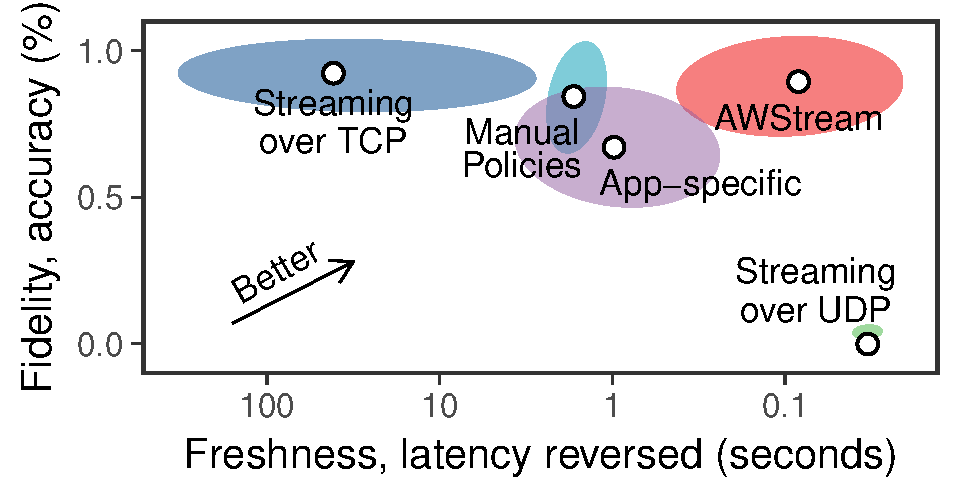
\includegraphics[width=0.8\columnwidth]{figures/figure1.pdf}
  \caption{The trade-off space between data freshness and fidelity when facing
    insufficient bandwidth (details in \autoref{sec:runtime-adaptation}).}
  \label{fig:intro}
  \vspace{-1em}
\end{figure}

Applications that simply use existing protocols without any attempt at
adaptation can result in extreme design points. For example, streaming over TCP
ensures reliable delivery (hence high fidelity) but backlogged data delays the
delivery of data (hence freshness suffers).  On the other hand, streaming over
UDP minimizes latency by sending packets as fast as possible, but uncontrolled
packet loss can devastate data fidelity.

Manual policies, such as sampling, allow developers to trade data fidelity for
freshness~\cite{rabkin2014aggregation}. However, it's difficult to write
accurate policies without extensive domain expertise or considerable effort. In
practice, developers write manual policies based on heuristics rather than
quantitative measurements and, as we show in \autoref{sec:evaluation}, such
policies can lead to sub-optimal performance in terms of both freshness and
fidelity.

Furthermore, application-specific optimizations often do not generalize. A
fine-tuned adaptation algorithm for one application works poorly for a different
application, if performance metrics or data distributions change.  For example,
video streaming focuses on quality of experience
(QoE)~\cite{michalos2012dynamic, pantos2016http, yin2015control}. Because humans
favor smoothness over image quality, these systems maintain a high frame rate
(e.g.,~\(25~\text{FPS}\)), and reduce the resolution under bandwidth limitation.
However, low resolution images can lead to poor accuracy for video analytics
that rely on the image details (e.g.,~face detection~\cite{viola2001rapid}).

In this paper, we present \sysname{}, a framework for building adaptive stream
processing applications that simultaneously simplifies development \emph{and}
improves application accuracy in the face of limited or varying wide-area
bandwidth.
% for the wide area that achieves low latency and high accuracy simultaneously
% with minimal developer effort.
\sysname{} achieves this with three novel contributions:

\begin{enumerate}[leftmargin=*, topsep=5pt]
\item \sysname{} introduces new programming abstractions by which a developer
  expresses \emph{what} degradation functions can be used by the framework.
  % {\bf Sylvia: Cut remainder of para? Too much detail for intro?}  More
  % specifically, \sysname{} augments existing stream processing operators with
  % a new \maybe{} operator. Its basic form takes a function that degrades the
  % input stream, and a list of values that serve as a knob to control the level
  % of degradation.  and . The knob specifies the degradation level that affects
  % data size and data fidelity.  We extend the basic form with a library of
  % specialized operators for common data types, such as
  % \texttt{maybe\_downsample} for images.  Our API is \textit{composable}
  % (multiple operators form a configuration that affects the adaptation
  % jointly), and \textit{extensible} (arbitrary functions and external
  % libraries can be embedded with our operators).
  Importantly, developers do not have to specify exactly when and how different
  degradation functions are to be used which is instead left to the \sysname{}
  framework.

\item Rather than rely on manual policies, \sysname{} automatically
  \emph{learns} a Pareto-optimal policy or strategy for when and how to invoke
  different degradation functions.  For this, we design a methodology that uses
  a combination of offline and online training to build an accurate model of the
  relationship between an application's accuracy and its bandwidth consumption
  under different combinations of degradation functions. Our solution exploits
  parallelism and sampling to efficiently explore the configuration space and
  learn an optimal strategy.

  % The key idea is to \textit{automatically} build an accurate and precise
  % \textit{performance model} instead of relying on manual policies or
  % application-specific optimizations.
  % We use an \textit{offline} process to bootstrap our system with
  % developer-supplied training data, and continuously refine the profile
  % \textit{online} to handle \textit{model drift}.  We exploit parallelism and
  % sampling-based techniques to efficiently explore the configuration space and
  % learn a adaptation strategy.

\item \sysname{}'s final contribution is the design and implementation of a
  runtime system that continually measures and adapts to network conditions.
  \sysname{} matches the streaming data rate to the measured available
  bandwidth, and achieves high accuracy by using the learned Pareto-optimal
  configurations.  Upon encountering network congestion, our adaptation
  algorithm increases the degradation level to reduce the data rate, such that
  no persistent queue builds up. To recover, it progressively decreases the
  degradation level after probing for more available bandwidth.

  % The runtime also provides additional options to control application
  % behaviors, such as limiting the maximum
  % allowed WAN bandwidth. For multiple applications, the profiles can be used
  % to allocate bandwidth among competing tasks for \textit{utility fairness}.
\end{enumerate}

We implement \sysname{} and use it to prototype three streaming applications:
augmented reality (AR), pedestrian detection (PD), and distributed Top-K
(TK). We use real-world data to profile these applications and evaluate their
runtime performance on a geo-distributed public cloud.  We show that
\sysname{}'s data-driven approach generates accurate profiles and that our
parallelism and sampling techniques can speed up profiling by up to 29$\times$
and 8.7$\times$ respectively.

With the combination of \sysname{}'s ability to learn better policies and its
well-designed runtime, our evaluation shows that \sysname{} significantly
outperforms non-adaptive applications: achieving a 40--100$\times$ reduction in
packet delivery times relative to applications built over TCP, or an over
45--88\% improvement in data fidelity (application accuracy) relative to
applications built over UDP. We also compare \sysname{} to
JetStream~\cite{rabkin2014aggregation}, a state-of-the-art system for building
adaptive streaming analytics that is based on manual policies. Our results show
that besides the benefit of generating optimal policies \textit{automatically},
\sysname{} achieves a 15-20$\times$ reduction in latency and 1-5\% improvement
in accuracy simultaneously relative to JetStream.

%%% Local Variables:
%%% mode: latex
%%% TeX-master: "../network"
%%% End:

%% LocalWords: VideoStorm analytics CDN CDNs geo IoT TCP UDP QoE runtime
%% LocalWords: GPUs TPUs downsample composable TK JetStream datacenter
\section{Motivation}
\label{sec:motivation}

In this section, we first examine the gap between high application demands and
limited WAN bandwidth. We then show that neither manual policies nor
application-specific optimizations solve the problem.

\subsection{Wide-area Streaming Applications}
\label{sec:wide-area-streaming}

We focus on wide-area streaming analytics, especially the emerging IoT
applications. We give two concrete examples.

\para{Video Surveillance.} We envisage a city-wide monitoring system
that aggregates camera feeds, from stationary ground cameras and
moving aerial vehicles, and analyzes video streams in real time for
surveillance, anomaly detection, or business
intelligence~\cite{oh2011large}. Recent advances in computer vision
have dramatically increased the accuracy for automatic visual scene
analysis, such as pedestrian detection~\cite{dollar2012pedestrian},
vehicle tracking~\cite{coifman1998real}, and facial recognition to
locate people of interest~\cite{lu2015surpassing,
  parkhi2015deep}. While some surveillance cameras use dedicated
links, an increasing number of surveillance systems, such as
Dropcam~\cite{dropcam} and Vigil~\cite{zhang2015design}, use the
public Internet and wireless links to reduce the cost of deployment
and management.

% \para{High-frequency IoT Sensors:} Although environmental sensors used to be
% slow and not data-intensive~\cite{atzori2010internet}, increasingly,
% high-frequency, high-precision sensors are deployed. For example, uPMUs
% monitor the electrical grid with a network of 1000 devices; each produces 12
% streams of 120 Hz high-precision values accurate to 100 ns. This amounts to
% 1.4 million points per second~\cite{andersen2016btrdb}.

\para{Infrastructure Monitoring.} Large organizations today are managing tens of
datacenters and edge clusters worldwide~\cite{calder2013mapping}. This
geo-distributed infrastructure continuously produces large volumes of data such
as data access logs, server monitoring logs, and performance
counters~\cite{alspaugh2014analyzing, pu2015low, vulimiri2015global}. While most
log analysis today runs in a batch mode on a daily basis, there is a trend
towards analyzing logs in real time for rapid
optimization~\cite{rabkin2014aggregation}. For example, CDNs can improve the
overall efficiency by optimizing data placement if the access logs can be
processed in real time. In Industrial IoT, large-scale real-time sensor
monitoring is becoming pervasive to detect anomalies, direct controls, and
predict maintenance ~\cite{balani2016enterprise, ge}.

%% ~\cite{xu2009detecting} We generated the HDFS logs by setting up a Hadoop
%% cluster on 203 EC2 nodes and running sample Hadoop map-reduce jobs for 48
%% hours, generating and processing over 200 TB of random data. We collected
%% over 24 million lines of logs from HDFS.

% We consider the practical issues with deploying these applications in the
% wide-area. Our stand is that these applications face a bigger network
% challenge.  Data generated from the edge often fail to be delivered to the
% processing site because of the scarce and variable bandwidth capacity in the
% wide-area. Once they arrive, existing stream processing systems can easily
% manage a large cluster and perform data analytics at real-time.

\subsection{Wide-area Bandwidth Characteristics}
\label{sec:wide-area-bandwidth}

WAN bandwidth is insufficient and costly, as shown by other
systems~\cite{hsieh17gaia, pu2015low, vulimiri2015wananlytics,
  vulimiri2015global}. Using Amazon EC2 as a case study, the WAN bandwidth
capacity is 15x smaller than their LAN bandwidth on average, and up to 60x
smaller in the worst case~\cite{hsieh17gaia}. In terms of pricing, the average
WAN bandwidth cost is up to 38x of the cost of renting two
machines~\cite{amazon2017pricing, hsieh17gaia}.

In addition to the scarcity and cost, the large variability of WAN bandwidth
also affects streaming workloads. We conducted a day-long measurement with
iPerf~\cite{iperf3} to study the pair-wise bandwidth between four Amazon EC2
sites (N. California, N. Virginia, Tokyo, Ireland).  The results show large
variance in almost all pairs---\autoref{fig:bw} is one such pair. There are
occasions when the available bandwidth is below 25\% of the maximum bandwidth.

\begin{figure}
  \centering
  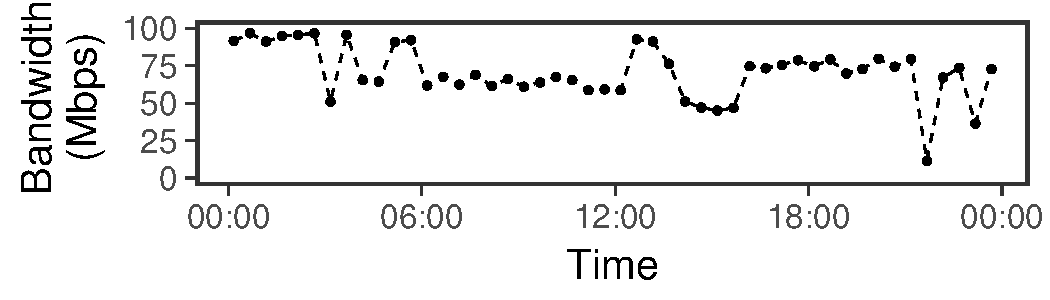
\includegraphics[width=0.9\linewidth]{figures/aws-variation.pdf}
  \caption{Bandwidth variations throughout the day between Amazon EC2 sites
    (from Ireland to California).}
  \label{fig:bw}
\end{figure}

The back-haul links between EC2 sites are better---if not at least
representative---in comparison to general WAN links. Similar scarcity and
variations exist in wireless networks~\cite{biswas2015large}, broadband access
networks~\cite{grover2013peeking, sundaresan2014bismark} and cellular
networks~\cite{nikravesh2014mobile}.

\subsection{Motivation for \awstream{}}
\label{subsec:motivation}

\pgfplotstableread[row sep=\\,col sep=&]{
  Frame Rate & Bandwidth (normalized) & Accuracy \\
  30 & 100 & 100 \\
  10 & 40 & 92 \\
  5 & 21 & 90 \\
  3 & 13 & 87 \\
  2 & 9 & 84 \\
}\stationaryframerate
\pgfplotstableread[row sep=\\,col sep=&]{
  Resolution & Bandwidth (normalized) & Accuracy \\
  1080p & 100 & 100 \\
  900p & 79 & 87 \\
  720p & 54 & 84 \\
  540p & 29 & 71 \\
  360p & 17 & 11 \\
}\stationaryresolution

\pgfplotstableread[row sep=\\,col sep=&]{
  Frame Rate & Bandwidth (normalized) & Accuracy \\
  30 & 100 & 100 \\
  10 & 65 & 64 \\
  5 & 46 & 32 \\
  3 & 34 & 18 \\
  2 & 27 & 10 \\
}\mobileframerate
\pgfplotstableread[row sep=\\,col sep=&]{
  Resolution & Bandwidth (normalized) & Accuracy \\
  1080p & 100 & 100 \\
  900p & 69 & 99 \\
  720p & 49 & 97 \\
  540p & 33 & 93 \\
  360p & 22 & 87 \\
}\mobileresolution

\captionsetup[subfigure]{
  justification=centering
}

\pgfplotsset{
  my bar/.style={%
    ybar,
    xtick pos=left,
    ytick pos=left,
    bar width               = .5cm,
    width                   = 1.0\textwidth,
    height                  = 0.18\textheight,
    xtick                   = data,
    enlarge x limits        = 0.15,
    nodes near coords,
    every node near coord/.append style={font=\footnotesize},
    nodes near coords align = {vertical},
    ymin                    = 0,
    ymax                    = 130,
    xlabel                  = {},
  }
}

\begin{figure}
  \centering
  \begin{tikzpicture}
    \begin{axis}[
      width = 4cm, height = 2cm, hide axis, xmin=0, xmax=1, ymin=0, ymax=1,
      legend style={ draw = none, legend columns= -1}, /tikz/every even
      column/.append style={column sep=0.2cm}, ] \addlegendimage{ybar, ybar
        legend, blue, fill=blue!50!white}\addlegendentry{B}
      \addlegendimage{ybar, ybar legend, red,
        fill=red!10!white}\addlegendentry{A} \legend{Bandwidth (normalized as
        \%), Accuracy (F1~\cite{van1979information} as \% based on
        IOU; see \autoref{fig:iou})}
    \end{axis}
  \end{tikzpicture}
  \\\vspace{1em}
  \begin{subfigure}{0.5\textwidth}
    \centering
    \textbf{Stationary Camera}
  \end{subfigure}%
  \begin{subfigure}{0.5\textwidth}
    \centering
    \textbf{Mobile Camera}
  \end{subfigure}
  \\\vspace{1em}
  \begin{subfigure}{0.5\textwidth}
    \centering
    \begin{tikzpicture}[scale=0.9]
      \begin{axis}[my bar,
        symbolic x coords = {30, 10, 5, 3, 2},
        ]

        \addplot [draw=blue, fill=blue!50!white, text=blue]
        table[x = Frame Rate, y = Bandwidth (normalized)]{\stationaryframerate};

        \addplot [draw=red, fill=red!10!white, text=red]
        table[x = Frame Rate, y = Accuracy]{\stationaryframerate};
        \legend{}
      \end{axis}
    \end{tikzpicture}
    \caption{Frame Rate (resolution = 1080p)}
    \label{fig:stationary-frame-rate}
  \end{subfigure}%
  \begin{subfigure}{0.5\textwidth}
    \centering
    \begin{tikzpicture}[scale=0.9]
      \begin{axis}[my bar,
        symbolic x coords = {30, 10, 5, 3, 2},
        ]
        \addplot [draw=blue, fill=blue!50!white, text=blue]
        table[x = Frame Rate, y = Bandwidth (normalized)]{\mobileframerate};

        \addplot [draw=red, fill=red!10!white, text=red]
        table[x = Frame Rate, y = Accuracy]{\mobileframerate};
        \legend{}
      \end{axis}
    \end{tikzpicture}
    \caption{Frame Rate (resolution = 1080p)}
    \label{fig:mobile-frame-rate}
  \end{subfigure}
  \\\vspace{1em}
  \begin{subfigure}{0.5\textwidth}
    \centering
    \begin{tikzpicture}[scale=0.9]
      \begin{axis}[my bar,
        symbolic x coords = {1080p, 900p, 720p, 540p, 360p},
        ]
        \addplot [draw=blue, fill=blue!50!white, text=blue]
        table[x = Resolution, y = Bandwidth (normalized)]{\stationaryresolution};

        \addplot [draw=red, fill=red!10!white, text=red]
        table[x = Resolution, y = Accuracy]{\stationaryresolution};
        \legend{}
      \end{axis}
    \end{tikzpicture}
    \caption{Resolution (frame rate = 30)}
    \label{fig:stationary-resolution}
  \end{subfigure}%
  \begin{subfigure}{0.5\textwidth}
    \centering
    \begin{tikzpicture}[scale=0.9]
      \begin{axis}[my bar,
        symbolic x coords = {1080p, 900p, 720p, 540p, 360p},
        ]
        \addplot [draw=blue, fill=blue!50!white, text=blue]
        table[x = Resolution, y = Bandwidth (normalized)]{\mobileresolution};

        \addplot [draw=red, fill=red!10!white, text=red]
        table[x = Resolution, y = Accuracy]{\mobileresolution};
        \legend{}
      \end{axis}
    \end{tikzpicture}
    \caption{Resolution (frame rate = 30)}
    \label{fig:mobile-resolution}
  \end{subfigure}
  \\\vspace{1em}
  \begin{subfigure}{0.5\textwidth}
    \centering
    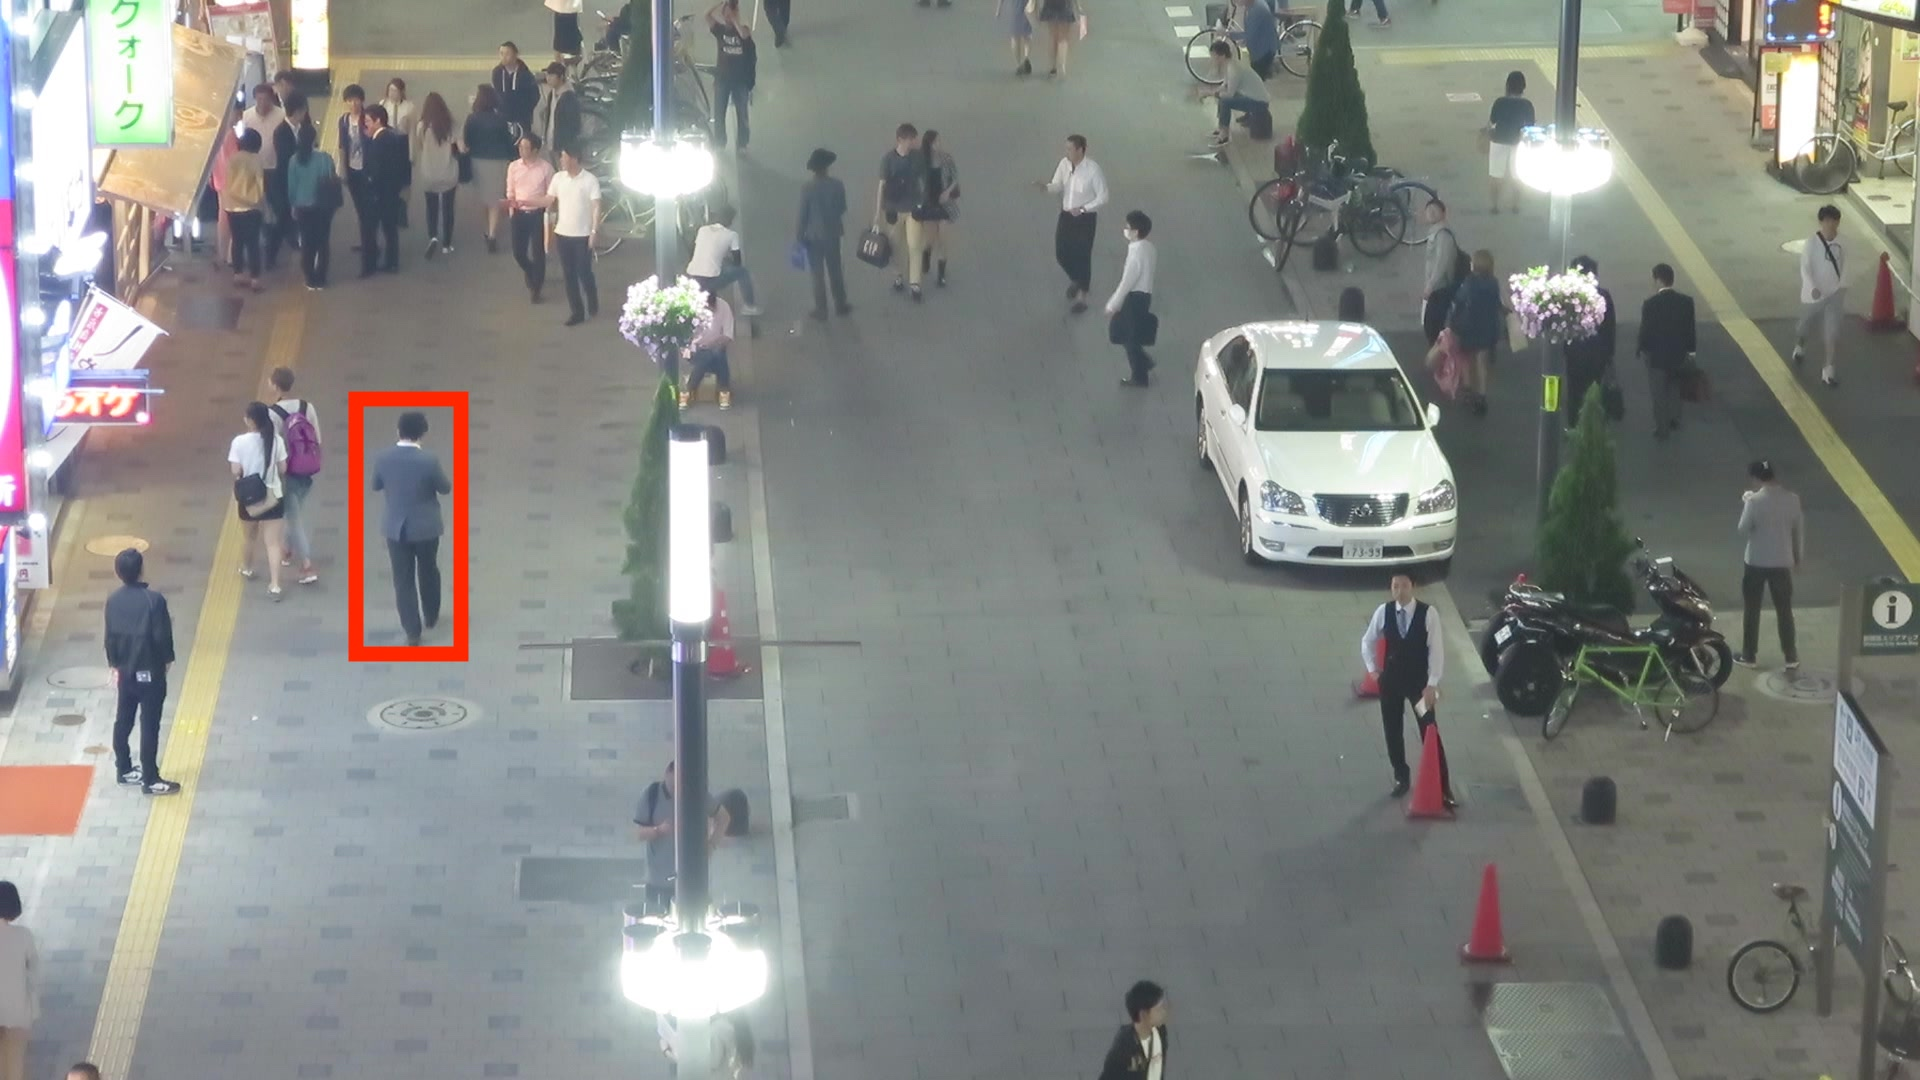
\includegraphics[width=0.8\textwidth]{figures/mot-1.jpg}
    \caption{t = 0s (small targets in far-field views)}
  \end{subfigure}%
  \begin{subfigure}{0.5\textwidth}
    \centering
    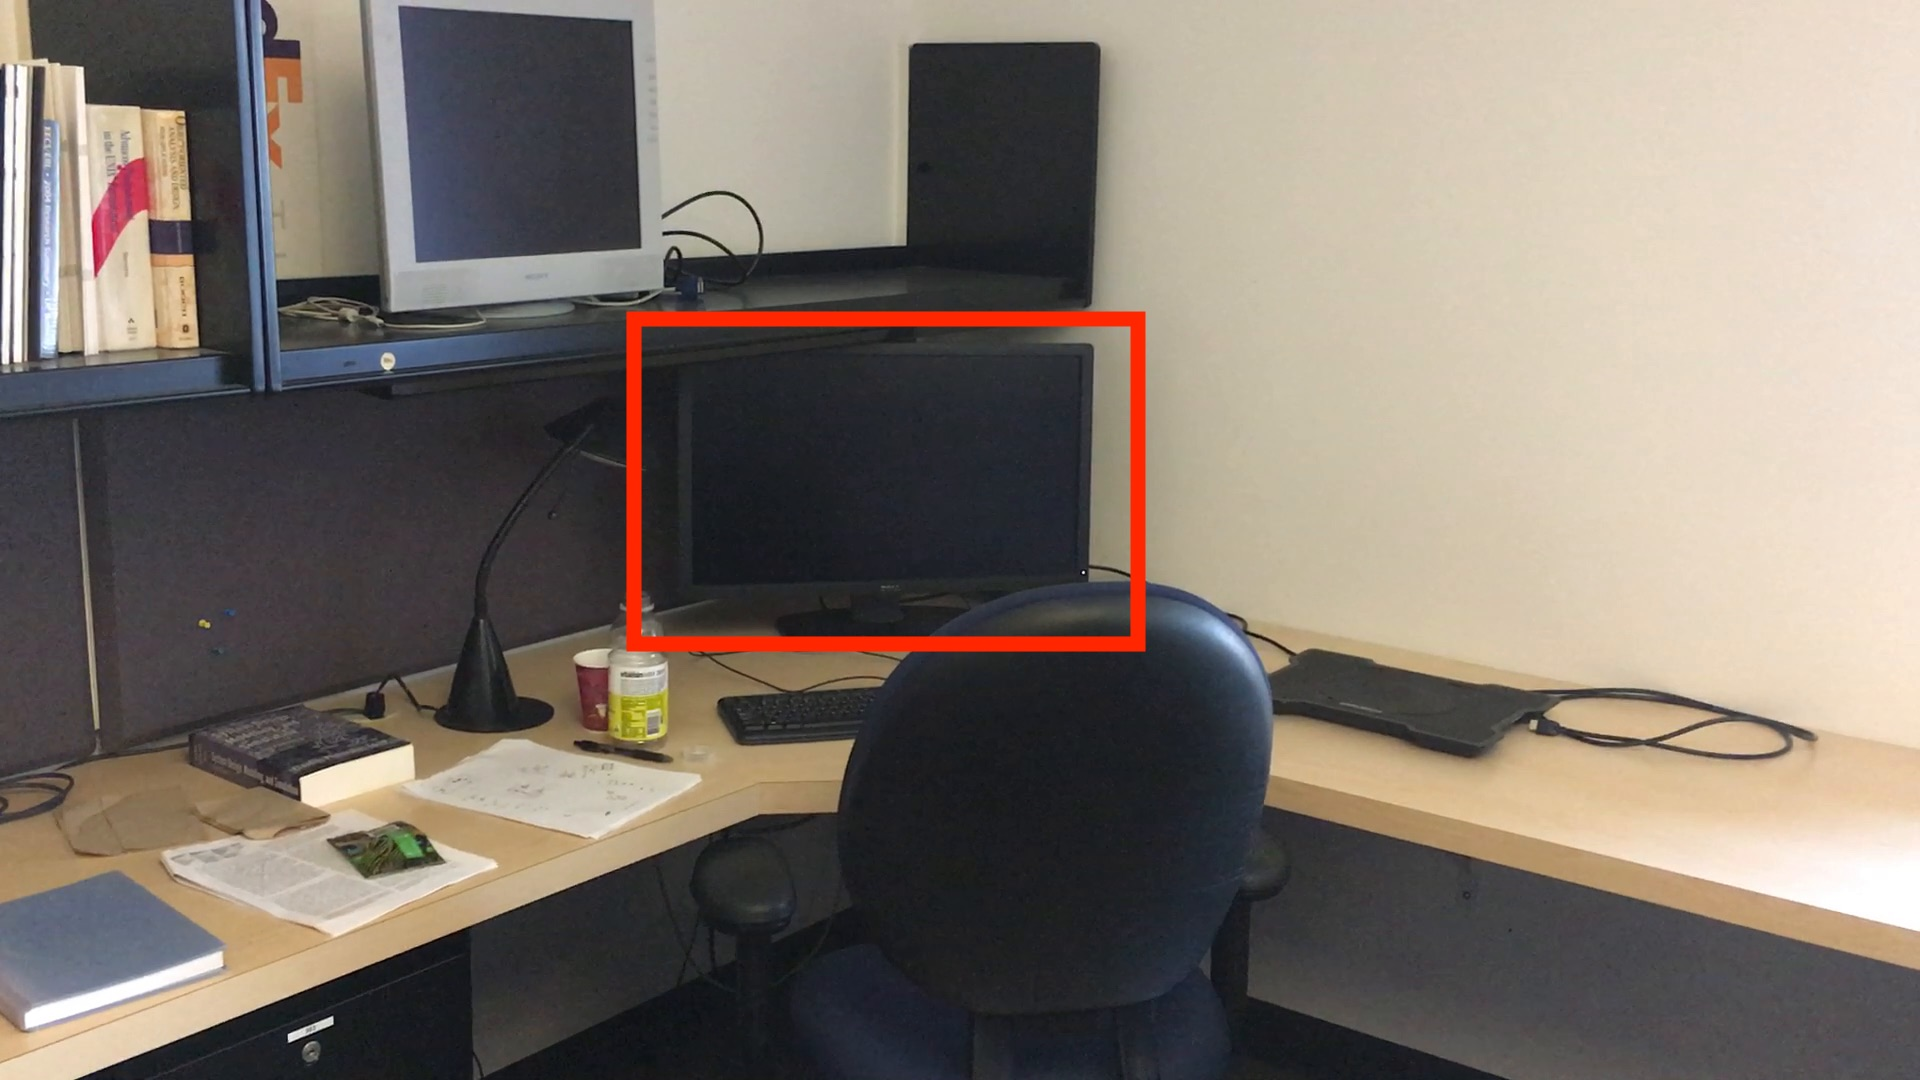
\includegraphics[width=0.8\textwidth]{figures/darknet-1.jpg}
    \caption{t = 0s (nearby and large targets)}
  \end{subfigure}
  \\\vspace{1em}
  \begin{subfigure}{0.5\textwidth}
    \centering
    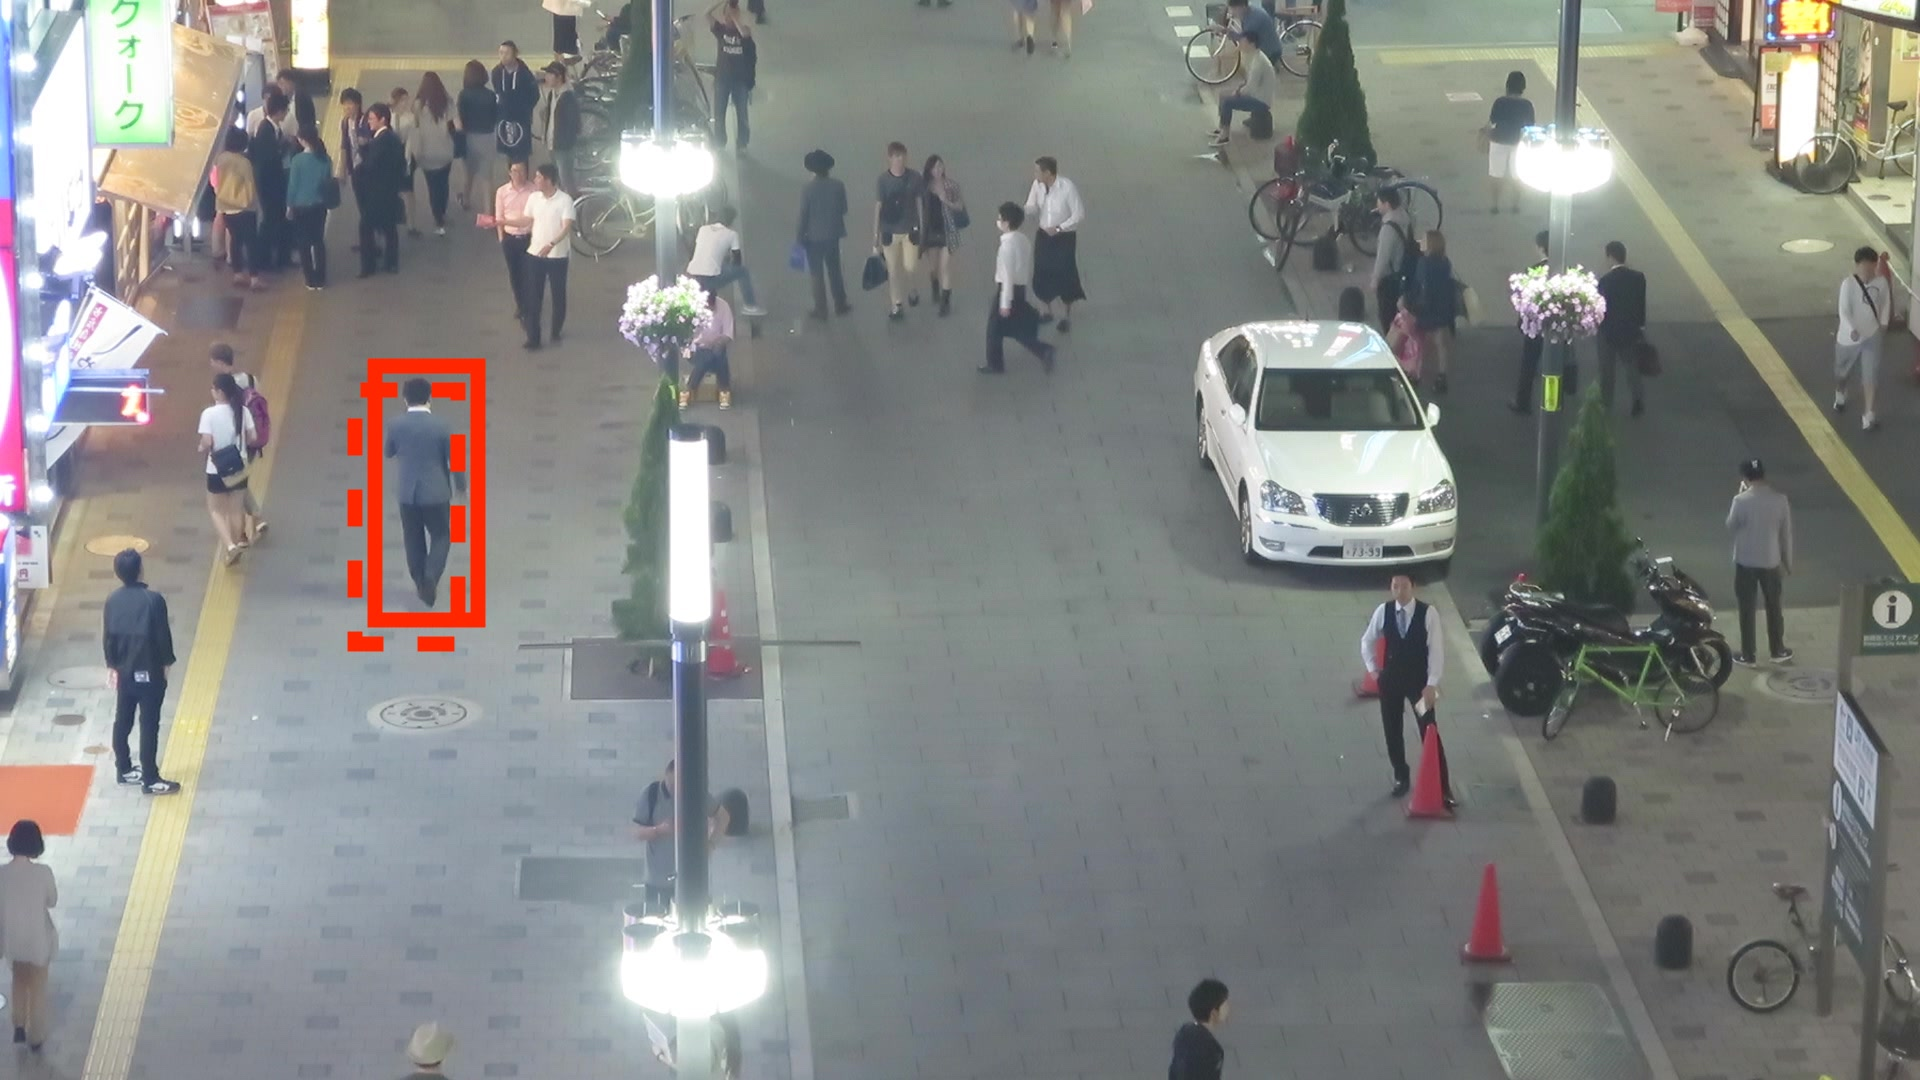
\includegraphics[width=0.8\textwidth]{figures/mot-2.jpg}
    \caption{t = 1s (small difference compared to t=0s)}
  \end{subfigure}%
  \begin{subfigure}{0.5\textwidth}
    \centering
    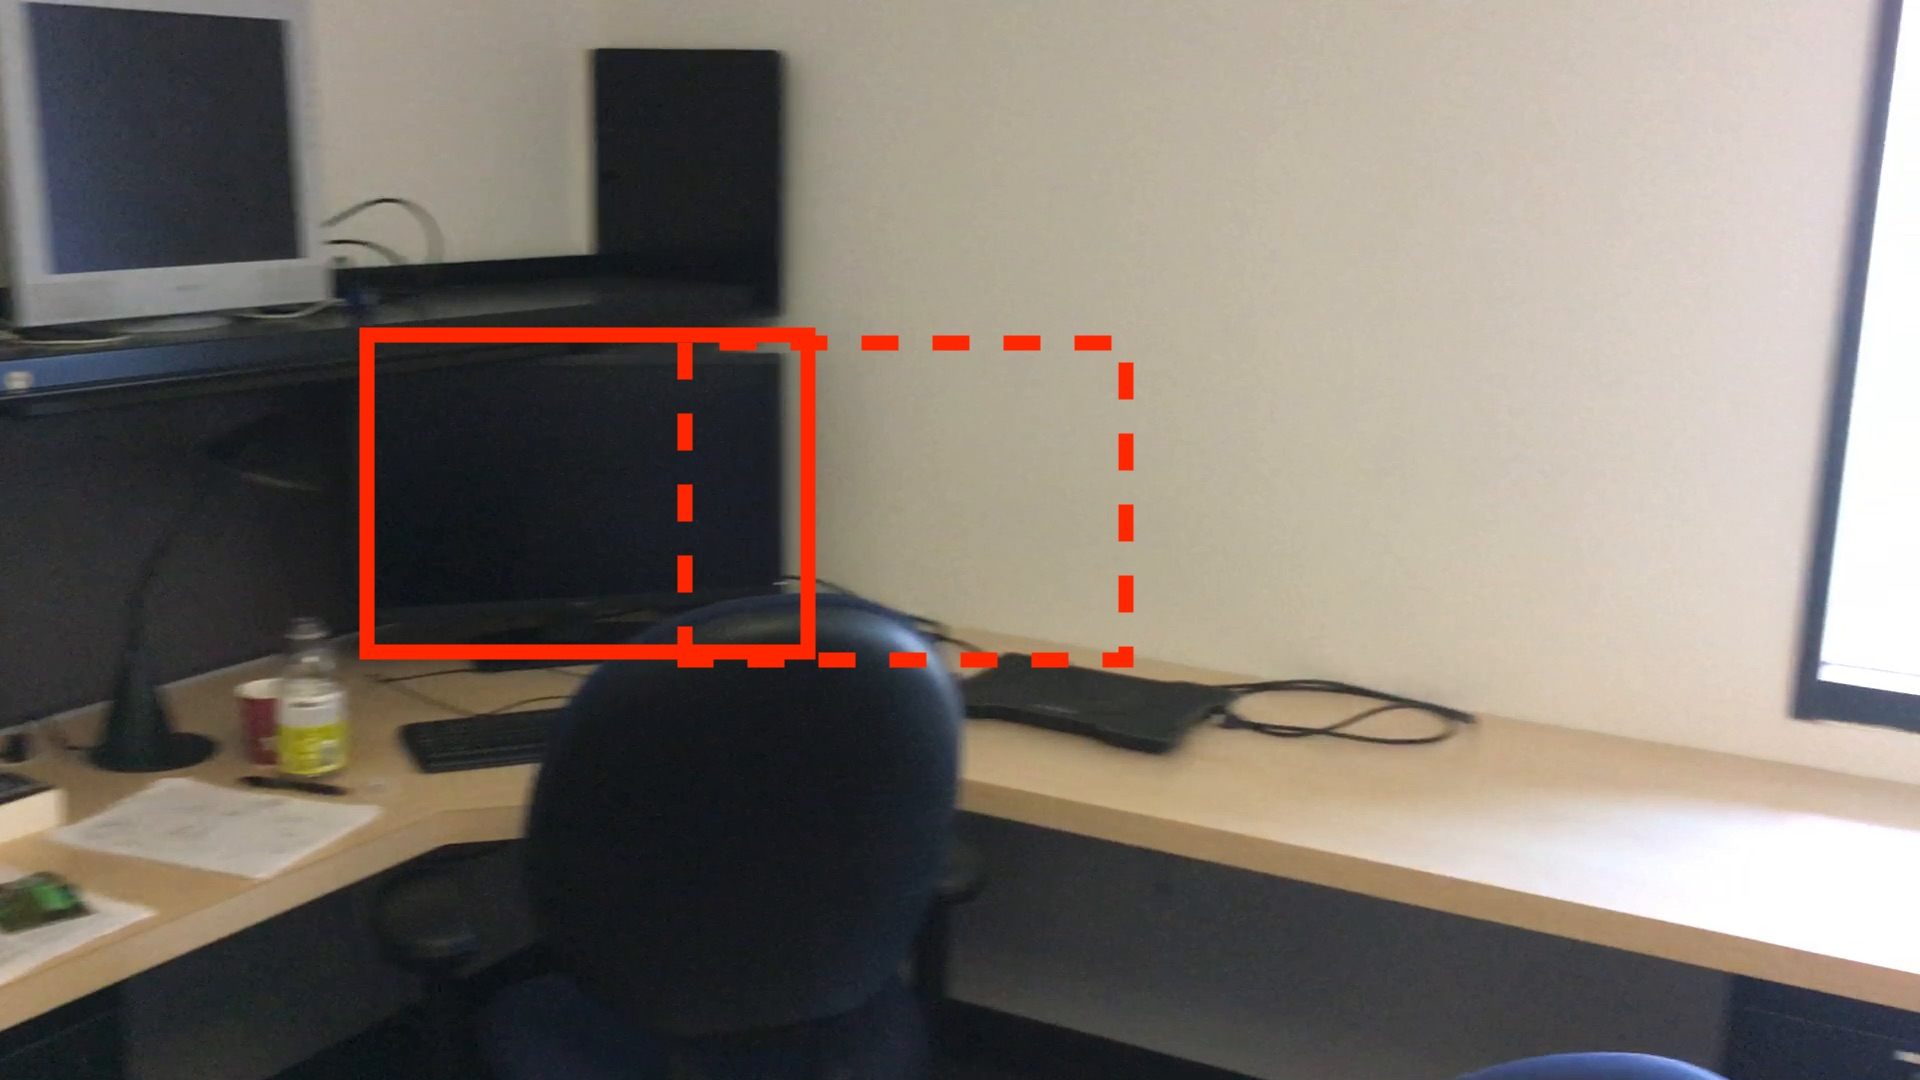
\includegraphics[width=0.8\textwidth]{figures/darknet-2.jpg}
    \caption{t = 1s (large difference compared to t=0s)}
  \end{subfigure}

  \caption{The measured bandwidth and application accuracy for two video
    analytics applications. (1) Manual policies lack precision without
    measurements and need to handle multiple dimensions, as in (a-b) and
    (c-d). (2) Application-specific optimizations do not generalize: degrading
    frame rates works well for stationary camera (a), but not for mobile camera
    (b). (e-h) shows example frames.}
  \label{fig:app-specific}
\end{figure}

%%% Local Variables:
%%% mode: latex
%%% TeX-master: "../network"
%%% End:


% \begin{figure*}
%   \centering
%   \includegraphics[width=0.85\linewidth]{figures/motiv-app-specific.pdf}
%   \caption{The measured bandwidth and application accuracy for two video
%     analytics applications. (1) Manual policies lack precision without
%     measurements and need to handle multiple dimensions (as in a-d). (2)
%     Application-specific optimizations do not generalize: degrading frame rates
%     works well for stationary camera (a), but not for mobile camera (c). (e-h)
%     shows example frames.}
%   \label{fig:app-specific}
% \end{figure*}

To address bandwidth limits, existing solutions use manual policies or
application-specific solutions. We discuss their drawbacks to motivate
\awstream{} (design in \autoref{sec:system}).

\para{Manual polices are sub-optimal.} JetStream~\cite{rabkin2014aggregation} is
the first to use degradation to address bandwidth limits in wide area. While
effective in comparison to non-adaptive systems, JetStream requires developers
to write manual policies, for example, ~\textit{``if bandwidth is insufficient,
  switch to sending images at 75\% fidelity, then 50\% if there still isn't
  enough bandwidth. Beyond that point, reduce the frame rate, but keep the image
  fidelity.''}\footnote{Excerpt from JetStream \S
  4.3~\cite{rabkin2014aggregation}.} We discuss the problems with manual
policies below and present quantitative evaluations in
\autoref{sec:runtime-adaptation}.

First, this policy is not accurate.  Developers write such rules based on
heuristics and do not back them up with measurements. Images with 75\% fidelity
do not necessarily lead to 75\% application accuracy. In terms of bandwidth,
naively one would think that reducing the frame rate by half will also half the
data rate. But if video encoding such as H.264~\cite{richardson2011h} is used, a
reduction in frame rate increases the inter-frame difference and creates
P-frames with larger sizes. \autoref{fig:mobile-frame-rate} shows that when
reducing the frame rate to 33\% (from \(30~\text{FPS}\) to \(10~\text{FPS}\)),
the bandwidth use can still be more than 50\%.

Second, it is not scalable to specify rules one by one. A fine-grain control
requires many rules in the policy. Besides, applications can degrade in multiple
dimensions and each dimension has different impacts (compare
\autoref{fig:stationary-frame-rate} with \autoref{fig:stationary-resolution}).
Specifying rules in detail and across dimensions manually is a tedious and
error-prone process.

Lastly, this abstraction is too low-level. It forces developers to study and
measure the impact of individual operations, prohibiting its wide adoption in
practice.

\para{Application-specific optimizations do not generalize.} Because each
application has different performance metrics and relies on different features,
a fine-tuned policy for one application will often work poorly for another. For
example, DASH~\cite{sodagar2011mpeg} optimizes QoE for video streaming; it keeps
a high frame rate and reduces resolutions for adaptation. Its policy that lowers
the resolution works poorly for video analytics that relies on image
details~\cite{lowe2004distinctive, viola2001rapid}. In
\autoref{fig:stationary-resolution}, we show that pedestrian detection accuracy
drops fast when reducing resolutions as pedestrian are small in the scenes.

Similar applications face different data distributions, as shown in
\autoref{fig:app-specific} between stationary cameras detecting pedestrians (up)
and mobile cameras recognizing objects (bottom). For stationary cameras, when we
consider the slow walking speed of pedestrians, a high frame rate is not
necessary. But high-resolution images are crucial because these surveillance
cameras are far away from the targets. In the mobile camera case, because the
camera moves, reducing the frame rate introduces significant errors.

%%% Local Variables:
%%% mode: latex
%%% TeX-master: "../network"
%%% End:

%% LocalWords: Dropcam IoT DCs geo CDNs iPerf JetStream scalable
%% LocalWords: bw runtime QoE analytics datacenters

\section{\sysname{} Design}
\label{sec:system}

To address the issues with manual policies or application-specific
optimizations, \sysname{} structures adaptation as a set of approximate,
modular, and extensible specifications (\autoref{sec:structure-adapt}). The
well-defined structure allows us to build a generic profiling tool that learns
an accurate relationship---we call it the profile---between bandwidth
consumption and application accuracy (\autoref{sec:automatic-profiling}). The
profile then guides the runtime to react with precision: achieving low latency
and high accuracy when facing insufficient bandwidth
(\autoref{sec:runtime}). \autoref{fig:overview} shows the high-level overview of
\sysname{}.

\begin{figure}
  \centering
  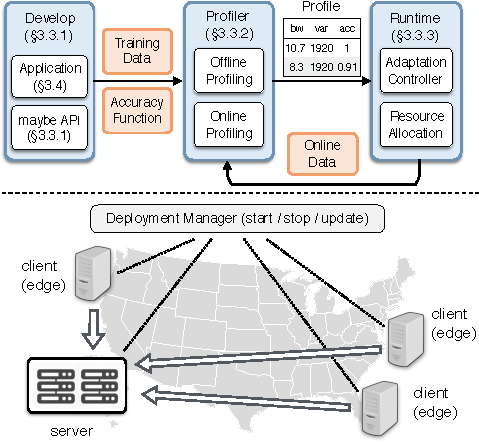
\includegraphics[width=\linewidth]{figures/system.pdf}
  \caption{\sysname{}'s phases: development, profiling, and runtime. \sysname{}
    also manages wide-area deployment.}
  \label{fig:overview}
\end{figure}

\subsection{API for Structured Adaptation}
\label{sec:structure-adapt}

\begin{table*}
  \small
  \centering
  \begin{tabular}{ c r l }
    \toprule
    \multirow{6}{*}{\shortstack{Normal \\ Operators}}
    & \textit{map} (f: I $\Rightarrow$ O) & Stream<I> $\Rightarrow$ Stream<O> \\
    & \textit{skip} (i: Int) & Stream<I> $\Rightarrow$
                                   Stream<I> \\
    & \textit{sliding\_window} (count: Int, f: Vec<I> $\Rightarrow$ O) & Stream<I> $\Rightarrow$
                                                                            Stream<O> \\
    & \textit{tumbling\_window} (count: Int, f: Vec<I> $\Rightarrow$ O) & Stream<I> $\Rightarrow$
                                                                            Stream<O> \\
    & \textit{timed\_window} (time: Duration, f: Vec<I> $\Rightarrow$ O) & Stream<I> $\Rightarrow$
                                                                            Stream<O> \\
    & ... & ... \\
    \midrule
    \multirow{5}{*}{\shortstack{Degradation\\Operators}}
    & \textit{maybe} (knobs: Vec<T>, f:  (T, I) $\Rightarrow$ I) & Stream<I> $\Rightarrow$
                                                                 Stream<I> \\
    & \textit{maybe\_skip} (knobs: Vec<Int>) & Stream<I> $\Rightarrow$ Stream<I> \\
    & \textit{maybe\_head} (knobs: Vec<Int>) & Stream<Vec<I>{}> $\Rightarrow$
                                                   Stream<Vec<I>{}> \\
    & \textit{maybe\_downsample} (knobs: Vec<(Int, Int)>) & Stream<Image> $\Rightarrow$ Stream<Image> \\
    & ... & ... \\
    \bottomrule
  \end{tabular}
  \vspace{0.2em}
  \caption{Stream processing operators in \sysname{}. \texttt{Vec<T>} represents
    a list of elements with type \texttt{T}.}
  \label{tab:operators}
\end{table*}

%% Introduce graphs of operators model
Most stream processing systems construct applications as a directed graph of
operators~\cite{toshniwal2014storm, zaharia2013discretized}. Each operator
transforms input streams into new streams. \sysname{} borrows the same
computation model and can support normal operators found in existing stream
processing systems such as JetStream~\cite{rabkin2014aggregation} (see example
operators in \autoref{tab:operators}).

To integrate adaptation as a first-class abstraction, \sysname{} introduces
\maybe{} operators that degrade data quality, yielding potential bandwidth
savings.  Our API design has three considerations. $(i)$~To free developers from
specifying exact rules, the API should allow specifications with
options. $(ii)$~To allow combining multiple dimensions, the API should be
modular. $(iii)$~To support flexible integration with arbitrary degradation
functions, the API should take user-defined functions. Therefore, our API is,

\begin{lstlisting}[xleftmargin=.2\textwidth]
maybe(knobs: Vec<T>, f: (T, I) => I)
\end{lstlisting}

We illustrate the use of the \texttt{maybe} operator with an example that
quantizes a stream of integers in Rust:

\begin{lstlisting}[xleftmargin=.1\textwidth]
let quantized_stream = vec![1, 2, 3, 4].into_stream()
    .maybe(vec![2, 4], |k, val| val.wrapping_div(k))
    .collect();
\end{lstlisting}

The snippet creates a stream of integers, chains a degradation operation, and
collects the execution result. In this example, the knob is [2, 4] and the
degradation function performs a wrapping (modular) division where the divisor is
the chosen knob. The knob value modifies the quantization level, affecting the
output: [1, 2, 3, 4] (no degradation), [0, 1, 1, 2] (k=2), or [0, 0, 0, 1]
(k=4). If the stream is then encoded---for example, run-length encoding as in
JPEG~\cite{wallace1992jpeg}---for transmission, the data size will depend on the
level of degradation.

Based on the \texttt{maybe} primitive, one can implement additional degradation
operators for common data types. For instance, \texttt{maybe\_head} will
optionally take the top values of a list; \texttt{maybe\_downsample} can resize
the image to a configured resolution. \sysname{} provides a number of such
operations as a library to simplify application development
(\autoref{tab:operators}).

With our API, the example mentioned in \autoref{subsec:motivation} can now be
implemented as follows:

\begin{lstlisting}[xleftmargin=.1\textwidth]
let app = Camera::new((1920, 1080), 30)
    .maybe_downsample(vec![(1600, 900), (1280, 720)])
    .maybe_skip(vec![2, 5])
    .map(|frame| frame.show())
    .compose();
\end{lstlisting}

This snippet first instantiates a \texttt{Camera} source, which produces
\texttt{Stream<Image>} with 1920x1080 resolution and 30 FPS\@. Two degradation
operations follow the source: one that downsamples the image to 1600x900 or
1280x720 resolution, and the other that skips every 2 or 5 frames, resulting in
30/(2+1)=10 FPS or 30/(5+1)= 6 FPS\@. This example then displays degraded
images. In practice, operators for further processing, such as encoding and
transmission, can be chained.

%%% Local Variables:
%%% mode: latex
%%% TeX-master: "../network"
%%% End:

%% LocalWords: UDFs Vec quantization quantized quantizes
%% LocalWords: downsample downsamples subsec resize

\subsection{Automatic Profiling}
\label{sec:automatic-profiling}

After developers use \maybe{} operators to specify potential degradation
operations, \awstream{} automatically builds an accurate profile. The profile
captures the relationship between \textit{application accuracy} and
\textit{bandwidth consumption} under different combinations of data degradation
operations. We describe the formalism, followed by techniques that efficiently
perform offline and online profiling.

\para{Profiling formalism.} Suppose a stream processing application has $n$
\maybe{} operators. Each operator introduces a knob $k_i$. The combination of
all knobs forms a \textit{configuration} $c = [k_{1}, k_{2}, ... k_{n}]$. The
set of all possible configurations $\mathbb{C}$ is the space that the profiling
explores. For each configuration $c$, there are two mappings that are of
particular interest: a mapping from $c$ to its bandwidth consumption $B(c)$ and
its accuracy measure $A(c)$. \autoref{tab:notations} summarizes these symbols.

\begin{table}
  \centering
  \begin{tabular}{r l}
    \toprule
    \textbf{Symbol} & \textbf{Description} \\
    \midrule
    $n$ & number of degradation operations \\
    $k_i$ & the \textit{i}-th degradation knob \\
    $c = [k_{1}, k_{2}, ... k_{n}]$ & one specific configuration \\
    $\mathbb{C}$ & the set of all configurations \\
    \midrule
    $B(c)$ & bandwidth requirement for $c$ \\
    $A(c)$ & accuracy measure for $c$ \\
    $\mathbb{P}$ & Pareto-optimal set \\
    \midrule
    $c_i$, $c_{i+1}$, $c_{\max}$ & current/next/maximal configuration at runtime \\
    $R$ & network delivery rate (estimated bandwidth) \\
    $\text{Q}_\text{E}$, $\text{Q}_\text{C}$ & messages when \texttt{Queue} is empty or congested \\
    $\text{R}_\text{C}$ & message when \texttt{Receiver} detects congestion \\
    $\text{AC}_\text{Probe}$ & message when \texttt{AC} requests probing \\
    $\text{S}_\text{ProbeDone}$ & message when \texttt{Socket} finishes probing \\
    \bottomrule
  \end{tabular}
  \caption{Notations used in this chapter.}
  \label{tab:notations}
\end{table}

The profiling looks for Pareto-optimal configurations; that is, for any
configuration $c$ in the Pareto-optimal set $\mathbb{P}$, there is no
alternative configuration $c'$ that requires less bandwidth and offers a higher
accuracy. Formally, $\mathbb{P}$ is defined as follows:

{\small \vspace{-1em}
  \begin{equation}
  \mathbb{P} = \{ c \in \mathbb{C} : \{ c' \in \mathbb{C}: B(c') < B(c),
  A(c') > A(c) \} = \varnothing\}
  \label{eq:pareto}
\end{equation}
}%

We show examples of knobs, configurations, and accuracy functions when we
present applications in \autoref{sec:implementation} and visualize the profile
of sample applications in \autoref{fig:all-profiles}.

\para{Offline Profiling.} We first use an offline process to build a bootstrap
profile (or default profile).  Because \awstream{} allows arbitrary functions as
the degradation functions, it does not assume a closed-form relationship for
$B(c)$ and $A(c)$. \awstream{} takes a data-driven approach: profiling
applications with developer-supplied training data. $B(c)$ is measured as the
data rate (bps) at the point of transmission. The accuracy $A(c)$ is measured
either against the groundtruth, or the reference results when all degradation
operations are off.

\awstream{} makes no assumptions on the performance models, and thus evaluates
all possible configurations.  While all knobs form a combinatorial space, the
offline profiling is only a one-time process.  We exploit parallelism to reduce
the profiling time.  Without any \textit{a priori} knowledge, all configurations
are assigned randomly to available machines.

% \para{Offline Profiling.} We first use an offline process to build a bootstrap
% profile (or default profile).  Because \awstream{} supports arbitrary
% degradation operations, we need to evaluate all combinations of the
% configurations offline profiling is a one-time process, \awstream{} currently
% performs an exhaustive evaluation of all configurations in $\mathbb{C}$
% despite all knobs form a combinatorial space. Future work could explore
% statistical methods to build performance models with a smaller number of
% training samples~\cite{venkataraman2016ernest, alipourfard2017cherrypick}.
% \awstream{} exploits parallelism when profiling all configurations.  Without
% any \textit{a priori} knowledge, all configurations are assigned randomly to
% all available machines.

\para{Online Profiling:} \awstream{} supports online profiling to continuously
refine the profile. The refinement handles \textit{model drift}, a problem when
the learned profile fails to predict the performance accurately. There are two
challenges with online profiling.  $(i)$~There are no ground-truth labels or
reference data to compute accuracy. Because labeling data is prohibitively labor
intensive and time consuming~\cite{russell2008labelme}, \awstream{} currently
uses raw data (data without degradation) as the reference. At runtime, if the
application streams raw data, it is used for online profiling. Otherwise, we
allocate additional bandwidth to transmit raw data, but only do so when there is
spare capacity. $(ii)$~Exhaustive profiling is expensive. If the profiling takes
too much time, the newly-learned profile may already be stale. \awstream{} uses a
combination of parallelization and sampling to speed up profiling, as below:

\begin{itemize}[leftmargin=*, topsep=3pt]

\item Parallelization with degradation-aware scheduling. Evaluating each
  configuration takes a different amount of time. Typically, an increase in the
  level of degradation leads to a decrease in computation; for example, a
  smaller FPS means fewer images to process. Therefore, we collect processing
  times for each configuration from offline profiling and schedule online
  profiling with longest first schedule (LFS)~\cite{karger2010scheduling} during
  parallelization.

\item Sampling-based profiling. Online profiling can speed up when we sample
  data or configurations. Sampling data reduces the amount of data to process,
  but at a cost of generating a less accurate profile. When sampling
  configuration, we can evaluate a subset of the Pareto-optimal configurations
  and compare their performances with an existing profile. A substantial
  difference, such as more than \SI{1}{Mbps} of bandwidth estimation, triggers a
  full profiling over all configurations to update the current profile.

\end{itemize}

%%% Local Variables:
%%% mode: latex
%%% TeX-master: "../network"
%%% End:

%% LocalWords: ProbeDone th combinatorial runtime parallelization priori
%% LocalWords: LFS mbps groundtruth

\subsection{Runtime Adaptation}
\label{sec:runtime}

At runtime, \sysname{} matches data rate to available bandwidth to minimize
latency and uses Pareto-optimal configurations to maximize accuracy. This
section focuses on the details of our runtime design. We defer the evaluation
and comparisons with existing systems (e.g.\,JetStream) to
\autoref{sec:runtime-adaptation}.

\begin{figure}
  \centering
  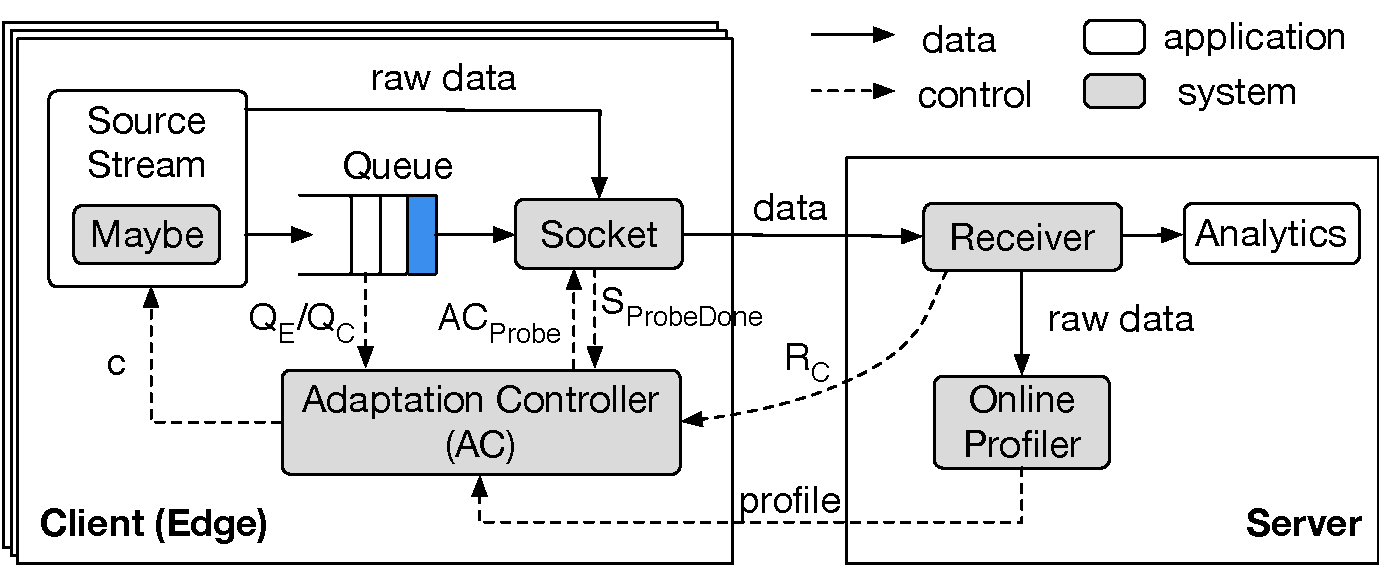
\includegraphics[width=\linewidth]{figures/runtime-adaptation.pdf}
  \caption{Runtime adaptation system architecture.}
  \label{fig:runtime}
\end{figure}

\autoref{fig:runtime} shows our runtime system architecture. \sysname{}
applications' source contains a \texttt{Maybe} module derived from all \maybe{}
operators. This module allows the controller to update the level of
degradation. Data generated by the source is then enqueued to \texttt{Queue} and
subsequently dequeued by \texttt{Socket}, which sends data over the network
using TCP. When the data generation rate exceeds \texttt{Socket}'s departure
rate, the queue grows. In this case, the adaptation controller (AC) queries the
estimated bandwidth from \texttt{Socket} and regulates the source stream by
updating the configuration. After the data is sent through the network,
\texttt{Receiver} delivers data to the application analytics. \texttt{Receiver}
also performs congestion detection and extracts raw data, if it is present.  It
tracks the minimal latency (similar to how BBR tracks
\texttt{RTprop}~\cite{cardwell2017bbr}) and reports sudden application-level
latency spikes to clients as congestion signals (\rc{}). If a new profile is
learned by the online profiler, it is fed back to AC for subsequent adaptation.

\autoref{fig:cc-sm} shows the adaptation algorithm with a state machine model
and \autoref{fig:cc-ex} shows the state transitions with an example. We first
describe all symbols. AC loads the profile and sorts all configurations with an
ascending order of bandwidth demand, resulting in a list
$[c_1, \dots, c_{\max}]$.  These configurations follow a total order:
$c_i < c_j$ if $B(c_i) < B(c_j)$.  We denote the current configuration as $c_i$
and the next $c_{i+1}$.  AC receives messages from other modules: \qe{} when
\texttt{Queue} is empty; $\text{Q}_\text{C}$ when queued items exceed a
threshold; and \rc{} when \texttt{Receiver} detects congestion. AC can query
\texttt{Socket} for delivery rate $R$ (arrow not shown) or request it to probe
($\text{AC}_{\text{Probe}}$) for a target bandwidth, often $B(c_{i+1})$. If
there is no congestion during the probing and $R > B(c_{i+1})$, \texttt{Socket}
sends back \spd{}. Below, we describe each state and transitions.

\begin{figure}
  \begin{subfigure}[t]{\columnwidth}
    \centering
    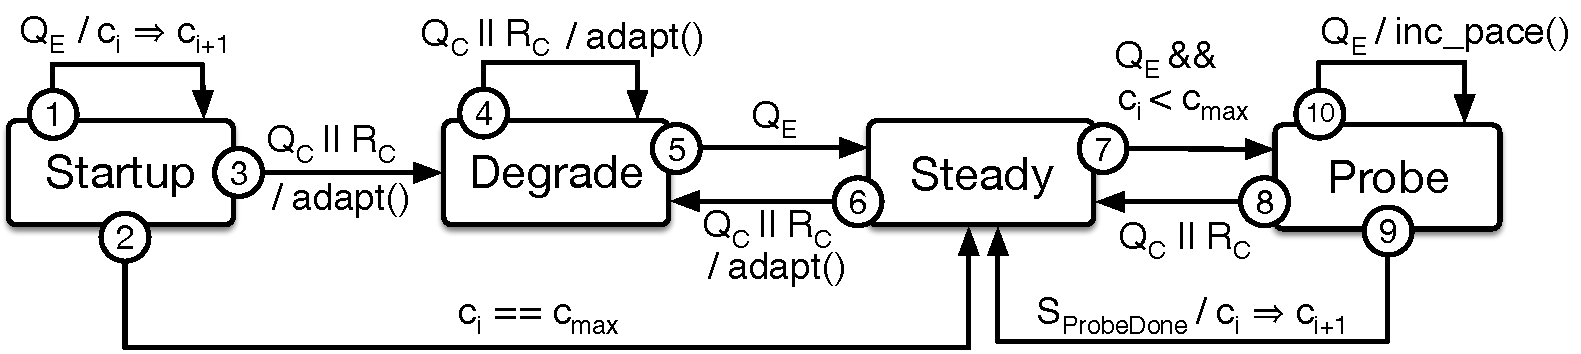
\includegraphics[width=\columnwidth]{figures/cc.pdf}
    \caption{Rate adaptation as a state machine.}
    \label{fig:cc-sm}
  \end{subfigure}
  \vspace{0.5em}
  \\
  \centering
  \begin{subfigure}[t]{\columnwidth}
    \centering
    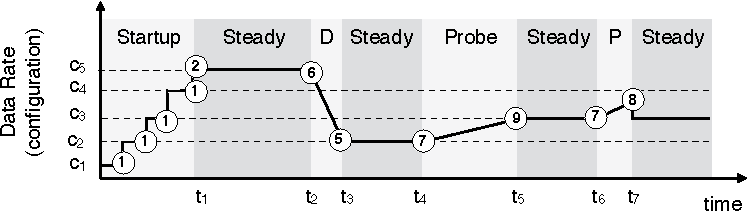
\includegraphics[width=0.9\columnwidth]{figures/cc2.pdf}
    \caption{An example illustrating the adaptation algorithm.}
    \label{fig:cc-ex}
  \end{subfigure}
  \caption{Runtime adaptation algorithm.}
  \label{fig:cc}
\end{figure}

\begin{itemize}[leftmargin=*, topsep=3pt, itemsep=0pt]

\item \textbf{Startup: rapid growth.} \sysname{} starts with $c_1$ and grows the
  rate ($c_i \Rightarrow c_{i+1}$) upon each \qe{}. The growth stops at
  $c_{\max}$ (to \texttt{Steady}) or if it receives \qc{}/\rc{} (to
  \texttt{Degrade}).

\item \textbf{Degrade: reacting to congestion.} Congestion is detected in two
  ways: (1) when \texttt{Queue} grows and exceeds a threshold, AC receives
  \qc{}; (2) when \texttt{Receiver} detects latency spikes, AC receives
  \rc{}. During congestion, AC runs the \texttt{adapt()} procedure by updating
  \texttt{Maybe} with the maximum-allowed $c$ that satisfies $B(c) < \alpha R$,
  where $\alpha \in (0, 1)$ and $R$ is \texttt{Socket}'s current delivery
  rate. A smaller $\alpha$ allows a quicker draining of the queue. After the
  congestion is resolved (\qe{} received), \sysname{} changes to
  \texttt{Steady}.

\item \textbf{Steady: low latency delivery.} \sysname{} achieves low latency by
  spending most of the time in \texttt{Steady}. It changes to \texttt{Degrade}
  when congestion occurs. If $c < c_{\max}$ and it receives \qe{}, AC starts
  \texttt{Probe} to check for more available bandwidth.

\item \textbf{Probe: more bandwidth for a higher accuracy.} Advancing $c_i$
  directly may cause congestion if $B(c_{i+1}) \gg B(c_i)$. To allow a smooth
  increase, AC requests \texttt{Socket} to probe by sending additional traffic
  controlled by \texttt{probe\_gain} (in \texttt{inc\_pace()}, similar to
  BBR~\cite{cardwell2017bbr}). Raw data is used for probing if available,
  otherwise we inject dummy traffic. \sysname{} stops probing under two
  conditions: (1) upon \spd{}, it advances $c_i$; (2) upon \qc{} or \rc{}, it
  returns to \texttt{Steady}. The explicit \texttt{Probe} phase stabilizes
  feedback loop and prevents oscillation.

\end{itemize}


\subsection{Resource Allocation \& Fairness}

In addition to rate adaptation, the profile is also useful for controlling a
single application's bandwidth usage or allocating resources among competing
tasks.

For individual applications, developers can pin-point a configuration for a
given bandwidth or accuracy goal. They can also specify a criterion to limit
effective configurations. For example, \sysname{} can enforce an upper bound on
the bandwidth consumption (e.g.,~do not exceed \SI{1}{Mbps}) or a lower bound on
application accuracy (e.g.,~do not fall below 75\%).

For multiple applications, their profiles allow novel bandwidth allocation
schemes such as utility fairness. Different from resource fairness with which
applications get an equal share of bandwidth, utility fairness aims to maximize
the \textit{minimal} application accuracy. With the profiles, bandwidth
allocation is equivalent to finding proper configuration $c^t$ for application
$t$. We formulate utility fairness as follows:

%% Pick one based on the space

\vspace{-0.5em}
\begin{equation}
  \vspace{-0.5em}
  \label{eq:multitask}
 \underset{c^t}{\max} \; \min({A^t(c^t)})
 \;
 \text{s.t.}
 \;
 \sum_t{B^t(c^t)} < R
\end{equation}

% \begin{equation}
%  \label{eq:multitask}
%  \begin{aligned}
%     & \underset{c^t}{\text{maximize}} & & \min({A^t(c^t)}) & & \\
%     & \text{subject to} & & \sum_t{B^t(c^t)} < R & & \\
%  \end{aligned}
% \end{equation}

Solving this optimization is computationally hard. \sysname{} uses heuristics
similar to VideoStorm~\cite{zhang2017live}: it starts with $c^t_1$ and improves
the application $t$ with the worst accuracy; this process iterates until all
bandwidth is allocated.

%%% Local Variables:
%%% mode: latex
%%% TeX-master: "../awstream"
%%% End:

%% LocalWords: runtime analytics enqueued dequeued TCP JetStream
%% LocalWords: RTprop BBR profiler sm VideoStorm

%%% Local Variables:
%%% mode: latex
%%% TeX-master: "../network"
%%% End:

\section{Implementation}
\label{sec:implementation}

While our proposed API is general and not language specific, we have implemented
\sysname{} prototype in Rust (\textasciitilde 4000 lines of code). \sysname{} is
open source on GitHub.\footnote{URL elided for anonymity.}  Applications use
\sysname{} as a library and configure the execution mode---profiling, runtime as
client, or runtime as server---with command line arguments.

% \begin{figure}
%   \centering
%   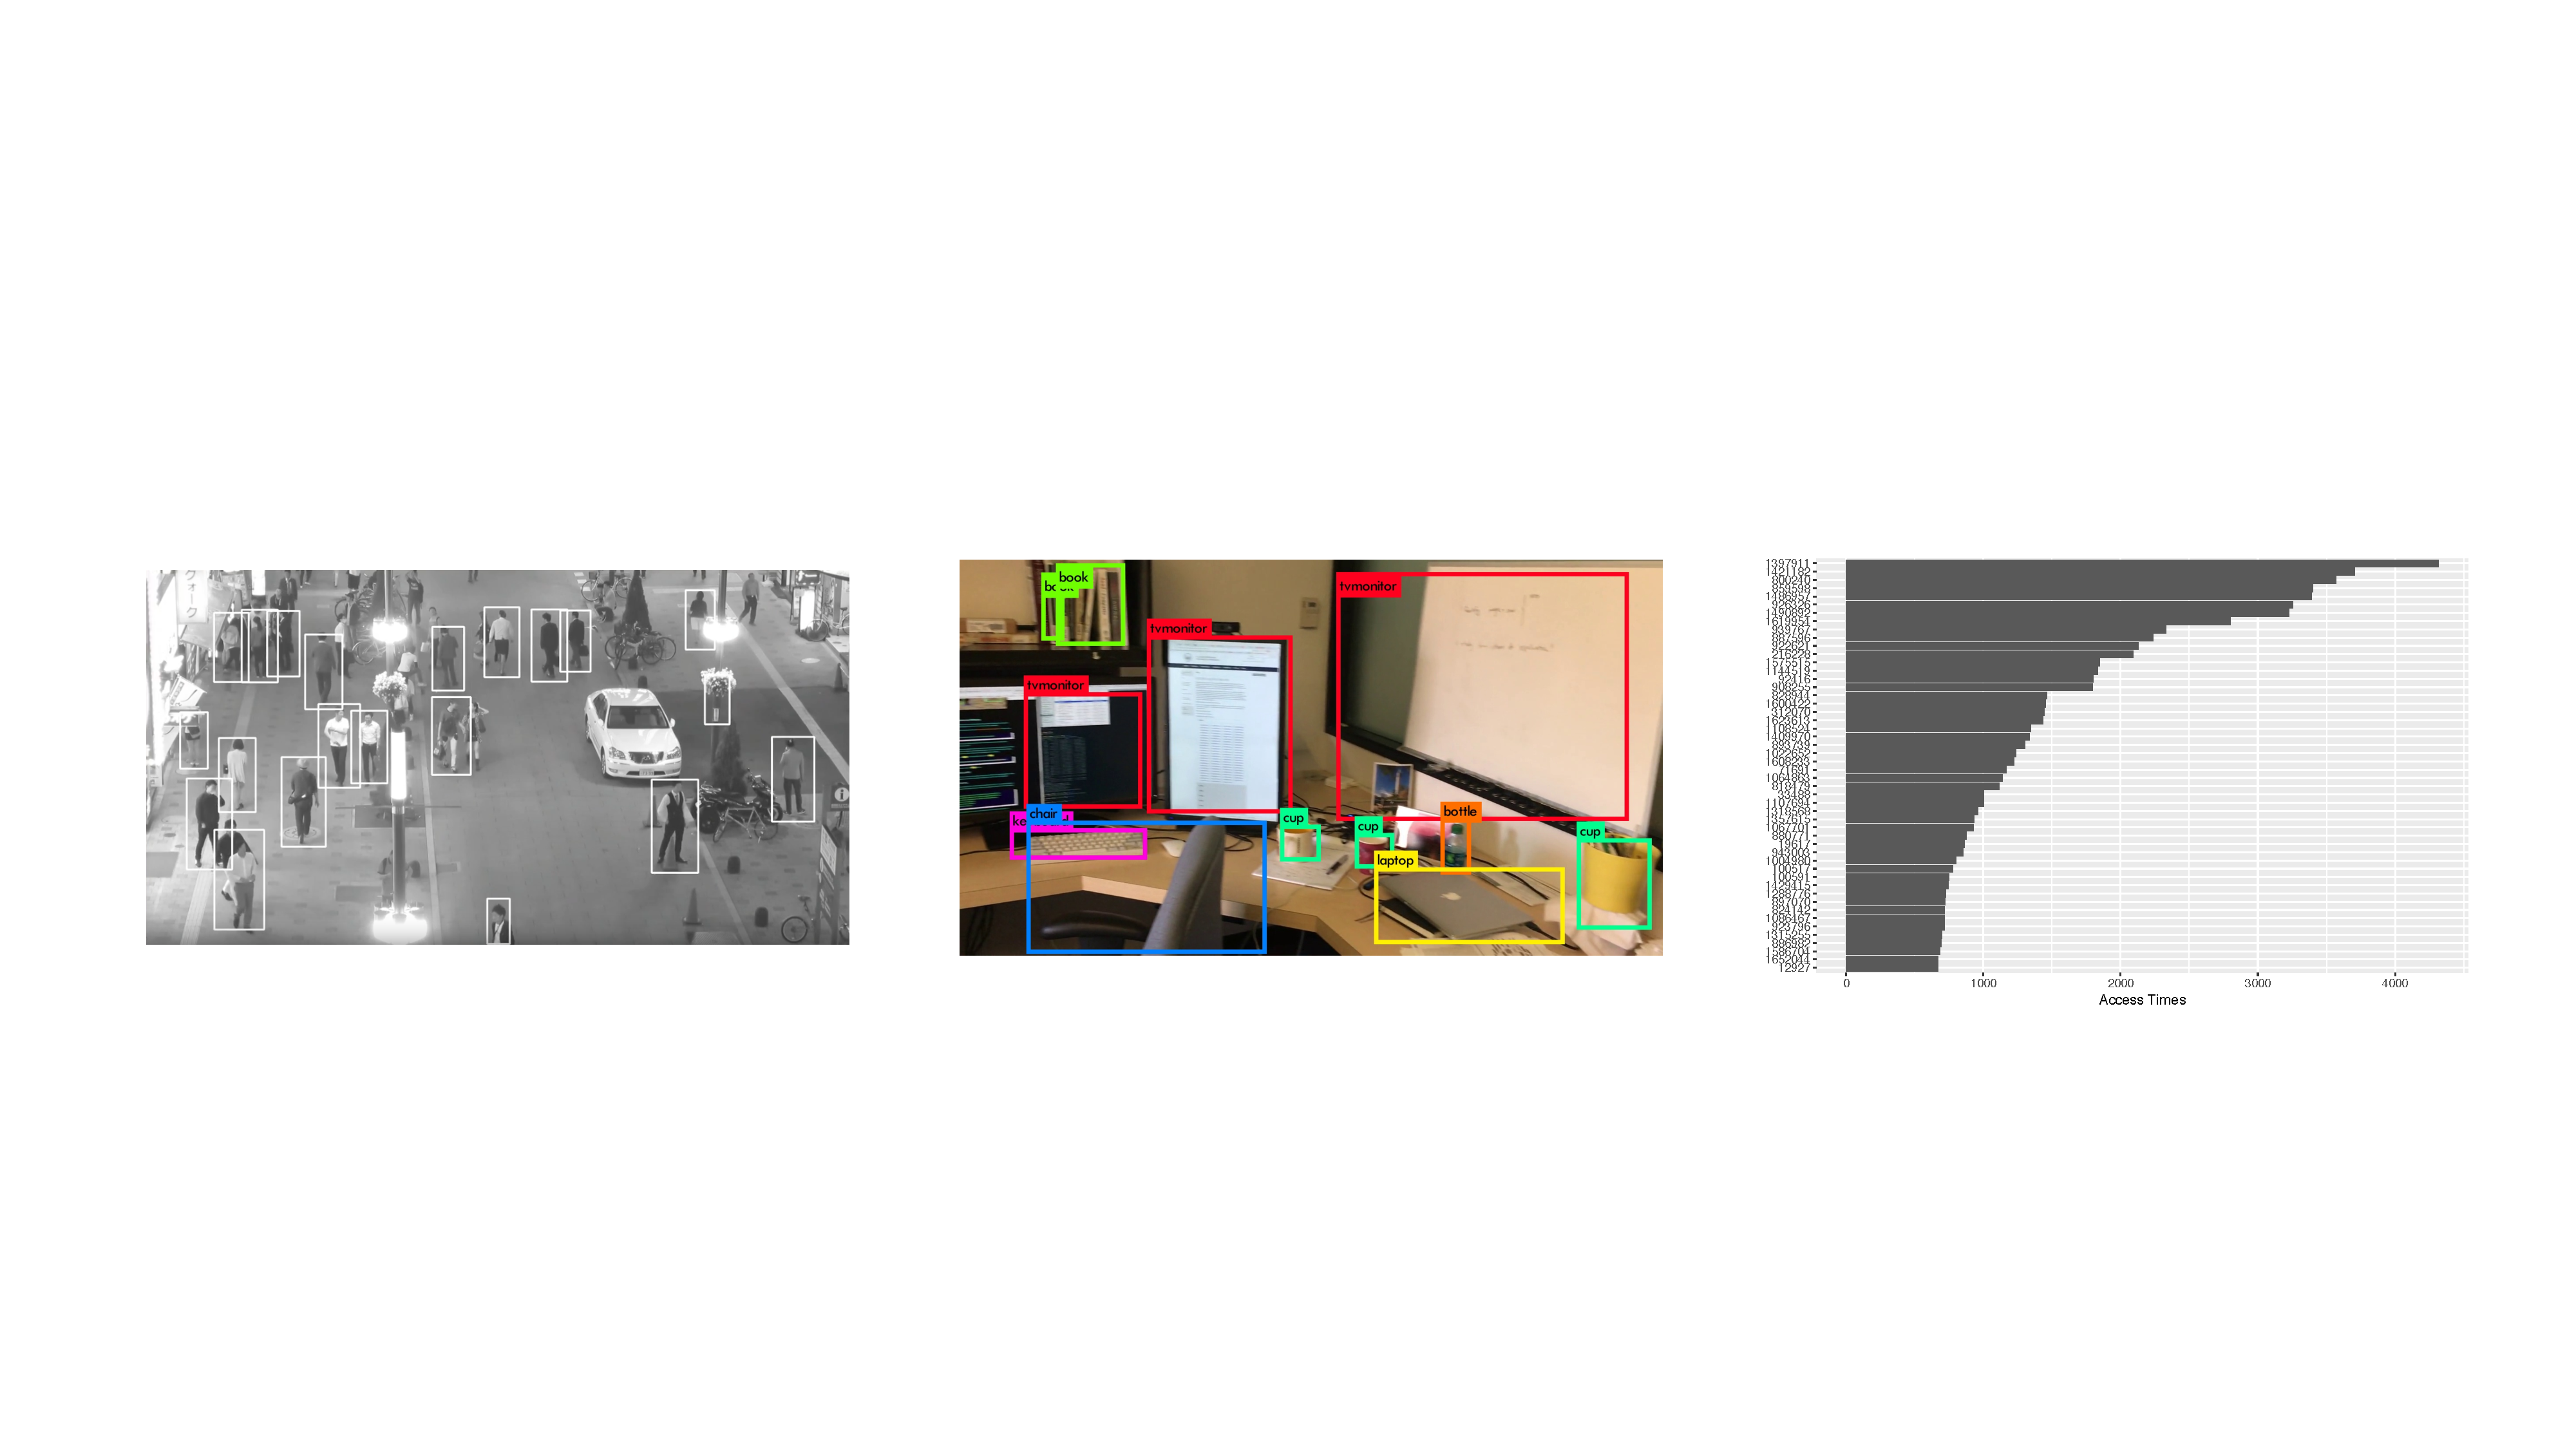
\includegraphics[width=\columnwidth]{figures/apps.pdf}
%   \caption{Three \sysname{} applications: augmented reality, pedestrian
%     detection, and distributed Top-K.}
%   \label{fig:three-apps}
% \end{figure}

\begin{table}
  \footnotesize
  \centering
  \begin{tabular}{c c c c}
    \toprule
    Application & Knobs & Accuracy & Dataset \\
    \midrule
    \specialcell{Augmented\\Reality}
                & \specialcell{resolution \\ frame rate \\ quantization }
                & F1 score~\cite{van1979information}
                & \specialcell{iPhone video clips\\training: office (24
    s)\\testing: home (246 s)} \\
    \midrule
    \specialcell{Pedestrian\\Detection}
                & \specialcell{resolution \\ frame rate \\ quantization }
                & F1 score
                & \specialcell{MOT16~\cite{milan2016mot16}\\training: MOT16-04\\testing: MOT16-03} \\
    \midrule
    \specialcell{Log Analysis\\(Top-K, K=50)}
                & \specialcell{head (N) \\ threshold (T) }
                & \specialcell{Kendall's $\tau$~\cite{abdi2007kendall}}
                & \specialcell{\href{https://www.sec.gov}{SEC.gov} logs~\cite{edgarlog} \\ training: 4 days \\
    testing: 16 days} \\
    \bottomrule
  \end{tabular}
  \vspace{0.5em}
  \caption{Application details.}
  \label{tab:apps}
  \vspace{-1em}
\end{table}

Using \sysname{}, we have built three applications: augmented reality (AR) that
recognizes nearby objects on mobile phones, pedestrian detection (PD) for
surveillance cameras, and a distributed log analysis to extract the Top-K mostly
accessed files (TK). \autoref{tab:apps} summarizes the application-specific
parts: knobs, accuracy functions, and datasets.

\para{Augmented Reality.} We target at augmented reality applications running on
mobile phones that recognize nearby objects by offloading the heavy computation
elsewhere, e.g.\,the cloud.

Our implementation uses OpenCV~\cite{opencvlibrary} for image-related operations
and YOLO~\cite{darknet13, redmon2016yolo9000}, a GPU-enabled pre-trained neural
network, for object recognition. Videos are encoded with
H.264~\cite{richardson2011h}. Our implementation uses GStreamer~\cite{gstreamer}
with \texttt{x264enc} plugin (\texttt{zerolatency} and constant quality). The
quantization factor affecting encoding quality becomes a knob in addition to
image resolutions and frame rates.

Object recognition returns a list of bounding boxes with the object type. Each
bounding box is a rectangle with normalized coordinates on the image. We compare
the detection against the reference result from raw data, and declare it success
if the intersection over union (IOU) is greater than
50\%~\cite{everingham2010pascal} and the object type matches. We use F1
score~\cite{Rijsbergen:1979:IR:539927} as the accuracy function. In terms of
dataset, we collected our own video clips: the training data is a 24-second long
video of an office environment; the test data is a 246-second long video of a
home environment.

\para{Pedestrian Detection.} This application analyzes streams of videos from
installed CCTV cameras and detects pedestrians inside. We use a similar setup
(OpenCV and GStreamer) as our augmented reality application except for the
analytical function. To detect pedestrians, we use GPU-accelerated histogram of
oriented gradients (HOG)~\cite{dalal2005histograms} with the default linear SVM
classifier from OpenCV. Because we do not recognize individual pedestrians, a
successful detection in this case only requires matching the bounding box. Our
evaluation uses MOT16 dataset~\cite{milan2016mot16} for both profiling and
runtime.

\begin{figure}
  \centering
  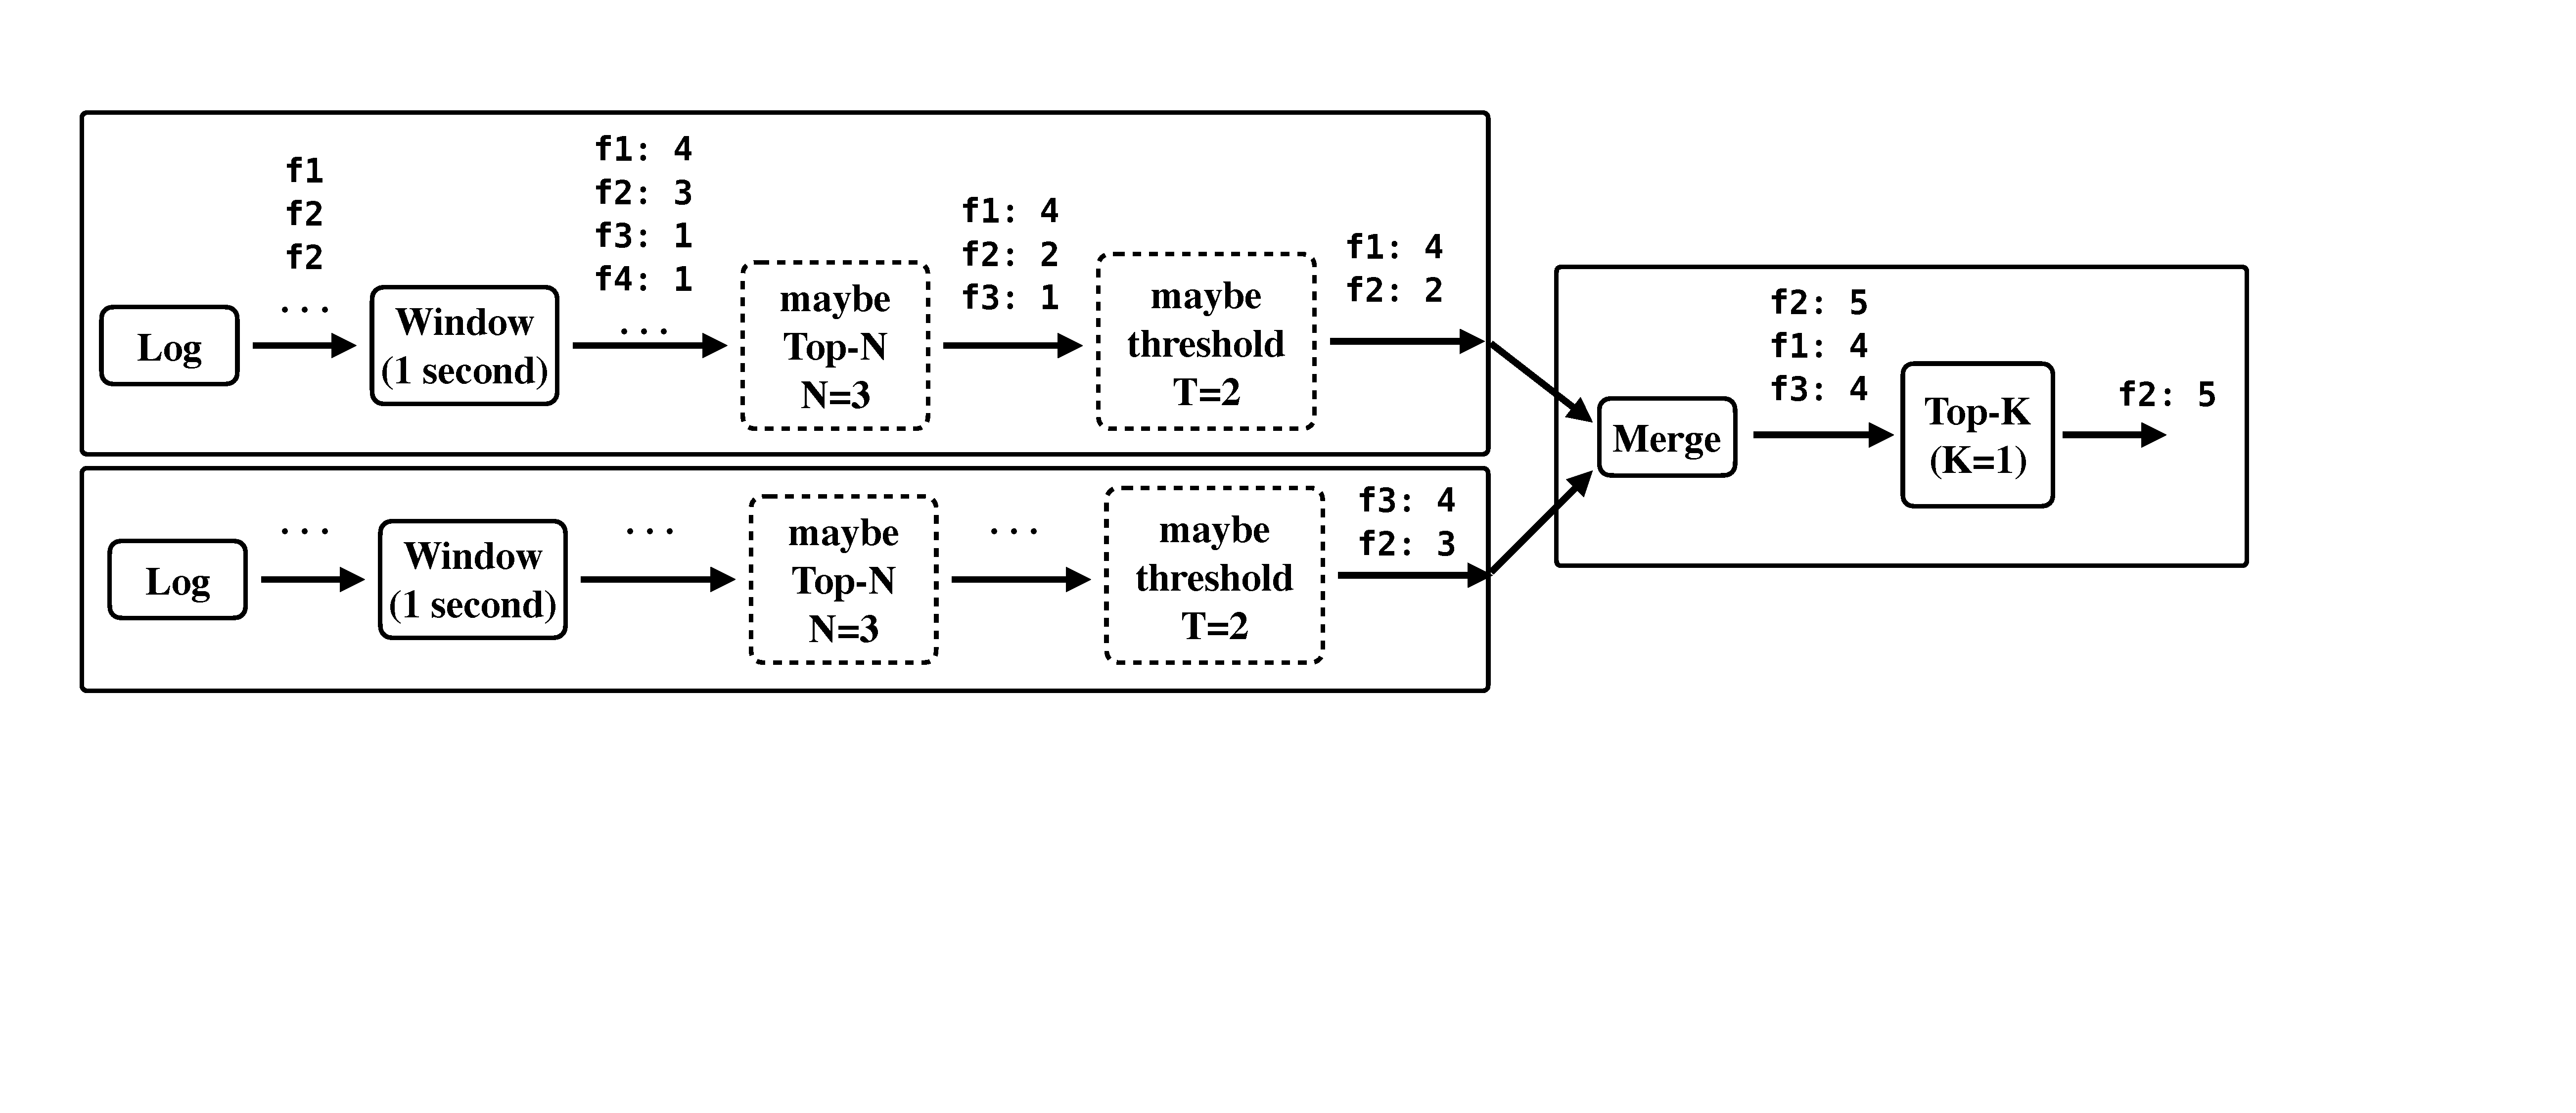
\includegraphics[width=\columnwidth]{figures/topk.pdf}
  \caption{A distributed Top-K application with two degradation operations:
    \texttt{head} and \texttt{threshold}. In this example, \texttt{f2}, which is
    not in Top-1 for either client, becomes the global Top-1 after the merge. It
    would have been purged if the clients use threshold T=3, demonstrating
    degradation that reduces data sizes affects fidelity.}
  \label{fig:topk}
  \vspace{-0.5em}
\end{figure}

\para{Distributed Top-K.} This application aggregates machine logs from
geo-distributed servers to find out the Top-K most accessed files, similar to
many Top-K queries~\cite{babcock2003distributed}.

\autoref{fig:topk} illustrates our processing pipeline with two degradation
operations. First each source node summarizes the log using \texttt{Window}
operator to reduce the data size, a pre-processing step. As many real-world
access patterns follow a long tail distribution, there can be a
large-but-irrelevant tail that contributes little to the final Top-K. Each
source node then filters the tail: (1) head(\texttt{N}) takes the top \texttt{N}
entries; (2) threshold(\texttt{T}) filters small entries whose count is smaller
than \texttt{T}. These two operations affect the final result and the exact
impact depends on data distribution. We implement these two operators by using
\sysname{}'s \maybe{} abstraction.

To measure the accuracy, we need to compare the correlation between two ranked
list. Kendall's~$\tau$~\cite{abdi2007kendall} is a correlation measure of the
concordance between two ranked list. The output ranges from \(-1\) to 1,
representing no agreement to complete agreement. To integrate with \sysname{},
we convert Kendall's~$\tau$ to [0, 1] with a linear transformation. For our
evaluation, we set K as 50 and use Apache log files that record and store user
access statistics for the \href{https://www.sec.gov}{SEC.gov} website. The logs
are split into four groups, simulating four geo-distributed nodes monitoring web
accesses. To match the load of popular web servers, we compress one hour's logs
into one second.

%%% Local Variables:
%%% mode: latex
%%% TeX-master: "../awstream"
%%% End:

%% LocalWords: runtime dataset quantization geo
\section{Evaluation}
\label{sec:evaluation}

In this section, we show the evaluations of \awstream{}, summarizing the results
as follows.

\begin{itemize}[leftmargin=1.5cm]
\item[\autoref{sec:application-profiles}] \awstream{} generates Pareto-optimal
  profiles across multiple dimensions with precision
  (\autoref{fig:all-profiles}).
\item[\autoref{sec:online-profiling}] Our parallel and sampling techniques
  speeds up offline and online profiling (\autoref{fig:parallel},
  \autoref{fig:online-tricks}).
\item[\autoref{sec:runtime-adaptation}] At runtime, \awstream{} achieves
  sub-second latency and nominal accuracy drop for all applications
  (\autoref{fig:ar-runtime}, \autoref{fig:pd-tk}) and across various network
  conditions (\autoref{fig:ar-rtt}).
\item[\autoref{sec:multi-task-alloc}] \awstream{} profiles allow different
  resource allocations: resource fairness and utility fairness
  (\autoref{fig:multitask}).
\end{itemize}

\subsection{Application Profiles}
\label{sec:application-profiles}

We run offline profiling using the training dataset described
in~\autoref{tab:apps} and show the learned profiles in
\autoref{fig:all-profiles}. In each figure, the cross dots represent the
bandwidth demand and application accuracy for one configuration. We highlight
the Pareto-optimal boundary $\mathbb{P}$ with blue dashed lines. To understand
each dimension's impact on the degradation, we highlight configurations from
tuning only \textit{one} dimension. From these profiles, we make the following
observations:

\begin{figure}
  \centering
  \begin{subfigure}[t]{0.45\textwidth}
    \centering
    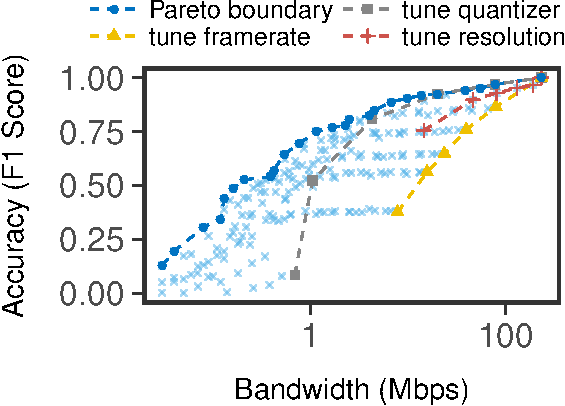
\includegraphics[width=\textwidth]{figures/profile-darknet.pdf}
    \caption{Augmented Reality (AR)}
    \label{fig:ar-profile}
  \end{subfigure}
  \hfill
  \begin{subfigure}[t]{0.45\textwidth}
    \centering
    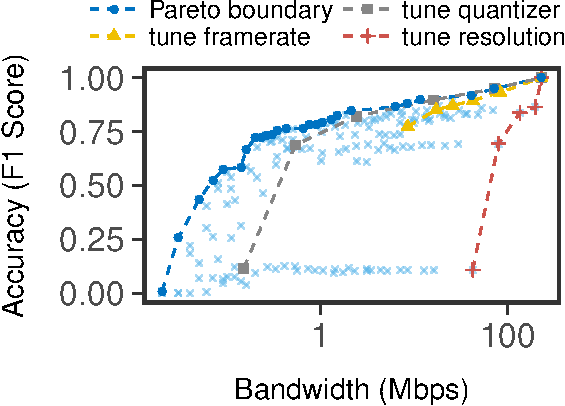
\includegraphics[width=\textwidth]{figures/profile-mot.pdf}
    \caption{Pedestrian Detection (PD)}
    \label{fig:pd-profile}
  \end{subfigure}
  \\
  \vspace{1em}
  \begin{subfigure}[t]{0.45\textwidth}
    \centering
    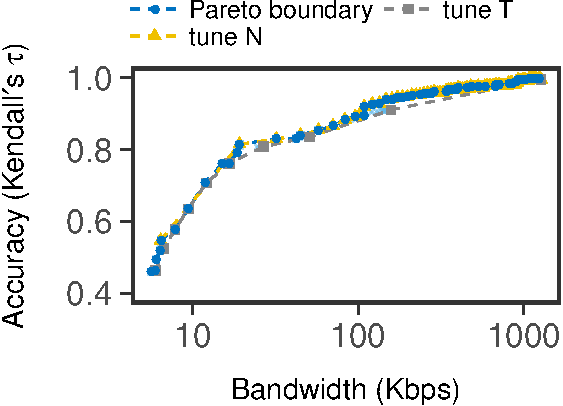
\includegraphics[width=\textwidth]{figures/profile-topk.pdf}
    \caption{Top-K (TK)}
    \label{fig:tk-profile}
  \end{subfigure}
  \caption{Application profiles of three applications. Each cross point is one
    configuration $c$'s performance $(B(c), A(c))$. All figures show the Pareto
    boundary as well as the performance if only tuning one dimension. Note the
    x-axis is in log scale.}
  \label{fig:all-profiles}
\end{figure}

\para{Large bandwidth variation.} For all three applications, The bandwidth
requirements of all three applications have two to three orders of magnitude of
difference (note the x-axis is in log scale). For AR and PD, the most expensive
configuration transmits videos at 1920x1080, 30 FPS and 0 quantization; it
consumes \SI{230}{Mbps}. In contrast to the large bandwidth variation, there is
a smaller variation in accuracy. In PD, for example, even after the bandwidth
reduces to \SI{1}{Mbps} (less than 1\% of the maximum), the accuracy is still
above 75\%. The large variation allows \awstream{} to operate at a high accuracy
configuration even under severe network deterioration.

\para{Distinct effects by each dimension.} Comparing dashed lines in each
profile, we see that the Pareto-optimal configurations are only achievable when
multiple knobs are in effect. Tuning only one dimension often leads to
sub-optimal performance. Within a single profile, the difference between tuning
individual dimensions is evident. For PD, tuning resolution (the red line) leads
to a quicker accuracy drop than tuning frame rate (the yellow line). Comparing
AR and PD, the same dimension has different impact. Tuning resolution is less
harmful in AR than PD; while tuning frame rate hurts AR more than PD\@. This
echoes our initial observation in~\autoref{subsec:motivation} that
application-specific optimizations do not generalize.

\para{Quantification with precision}. The generated profiles are actionable
configurations that control the knobs with precision. For example, if PD
transmits video at 1920x1080 resolution, \(10~\text{FPS}\) and a quantization of
20, it will consume 11.7 mbps of bandwidth, achieving roughly 90\%
accuracy. This saves developers from laboriously analyzing their application to
compute manual policies.

\subsection{Profiling Efficiency \& Online Profiling}
\label{sec:online-profiling}

This section focuses on the AR application as a case study; our profiling
techniques---parallelism and sampling---do not make assumptions about the
application; therefore, the evaluation results can be generalized to other
applications.

In AR, there are 216 different configurations: 6 resolutions, 6 frame rates and
6 quantization levels. AR uses YOLO~\cite{redmon2016yolo9000}, a neural network
model for object detection. It takes roughly \SI{30}{\ms} to process one frame
on GeForce\textregistered\space GTX 970.\footnote{YOLO resizes images to fixed
  416$\times$416 resolutions as required by the neural network. Evaluating
  images with different resolutions takes similar time.}  But different
configurations require different times for processing. For example, a
\(10~\text{FPS}\) video has 1/3 of the frames to process in comparison to a
\(30~\text{FPS}\) video.  In our experiment, to evaluate all 216 configurations,
it takes 52 seconds for 1 second worth of data. We denote such overhead as
52X\@. \hyperref[sec:automatic-profiling]{Section 3.2} discusses parallel and
sampling techniques to improve the profiling efficiency; we present their
evaluations as follows.

\begin{figure}
  \centering
  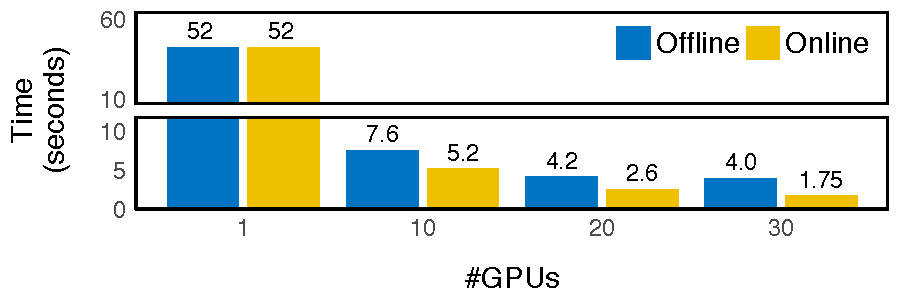
\includegraphics[width=0.8\columnwidth]{figures/parallel.pdf}
  \vspace{-1em}
  \caption{Parallelism speeds up both offline and online profiling.  The y-axis
    shows the profiling time for 1-second video.}
  \label{fig:parallel}
  \vspace{-0.5em}
\end{figure}

\para{Parallelism reduces the profiling time (\autoref{fig:parallel})}. Because
evaluating each individual configuration is independent of other configurations,
we parallelize the profiling task by assigning configurations to GPUs.
$(i)$~Our offline profiling assigns configurations randomly.  With the increased
number of GPUs, the overhead reduces from 52X to 4X with 30 GPUs.  $(ii)$~Our
online profiling assigns configurations based on the processing times collected
during offline.  \awstream{} uses LFS~\cite{karger2010scheduling} to minimize the
makespan and reduces the overhead to 1.75X with 30 GPUs (29$\times$ gain).

\para{Sampling techniques speed up online profiling
  (\autoref{fig:online-tricks}).}  Before we evaluate the speed up, we validate
\textit{model drift} with real-world data. When using the profile trained in an
office environment, the application should use a configuration of 1280x720,
\SI{30}{FPS} and 20 quantization to meet an \SI{11}{Mbps} goal. We test it
against a home environment; but at about t=100s, the camera points out of the
window to detect objects on the street. Because of the scene change, the
configuration fails to predict bandwidth, as illustrated in
\autoref{fig:offline}.

To correct the profile, if we continuously run the profiling online and update
the profile, the application will choose the right configuration to meet the
bandwidth limit.  \autoref{fig:online} shows the bandwidth prediction when we
continuously profile with the past 30 seconds of video. At time t=120s, the new
prediction corrects the drift. The downside of continuous profiling, as
discussed earlier, is the cost: 52X overhead with 1 GPU\@. In addition to
parallelism, \awstream{} uses sampling techniques for online profiling
(improvements in \autoref{tab:online}):

(i) Partial data. Instead of using all the past data, we run profiling with only
a fraction of the raw data.  \autoref{fig:online-partial} shows the bandwidth
consumption if the profiling uses only 10 seconds of data out of the past 30
seconds. In this way, although the profile may be less accurate (the
mis-prediction at t=80-100s), and there is a delay in reacting to data change
(the mis-prediction is corrected after t=125s), we save the online profiling by
3$\times$ (from 52X to 17X).

(ii) Partial configurations. If we use the past profile as a reference and only
measure a subset of $\mathbb{P}$, the savings can be substantial. A full
profiling is only triggered if there is a significant
difference. \autoref{fig:online-trigger} shows the bandwidth prediction if we
evaluate 5 configurations continuously and trigger a full profiling when the
bandwidth estimation is off by \SI{1}{Mbps} or the accuracy is off by 10\%.  For
our test data, this scheme is enough to correct model drifts by predicting an
accurate bandwidth usage (compare \autoref{fig:online} and
\autoref{fig:online-trigger}).  The overhead reduces to 6X because we run full
profiling less often (only two full profiling). It is an 8.7$\times$ gain.

\begin{figure}
  \centering
  \begin{subfigure}[t]{0.5\columnwidth}
    \centering
    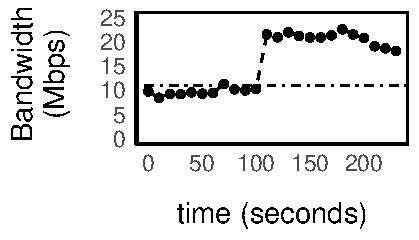
\includegraphics[width=0.85\textwidth]{figures/online1.pdf}
    \caption{Offline only}
    \label{fig:offline}
  \end{subfigure}%
  \begin{subfigure}[t]{0.5\columnwidth}
    \centering
    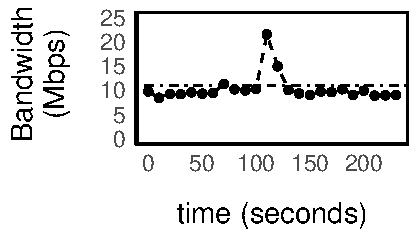
\includegraphics[width=0.85\textwidth]{figures/online2.pdf}
    \caption{Online (continuous)}
    \label{fig:online}
  \end{subfigure}
  \\
  \vspace{0.5em}
  \begin{subfigure}[t]{0.5\columnwidth}
    \centering
    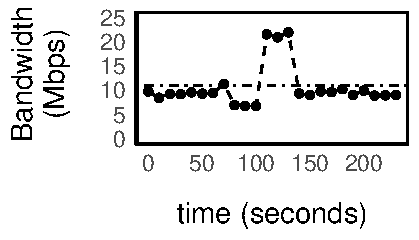
\includegraphics[width=0.85\textwidth]{figures/online3.pdf}
    \caption{Partial data}
    \label{fig:online-partial}
  \end{subfigure}%
  \begin{subfigure}[t]{0.5\columnwidth}
    \centering
    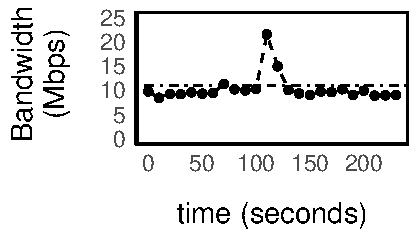
\includegraphics[width=0.85\textwidth]{figures/online4.pdf}
    \caption{Partial configurations}
    \label{fig:online-trigger}
  \end{subfigure}
  \caption{The horizontal reference line is the target bandwidth
    (\SI{11}{Mbps}). (1) Online profiling is necessary to handle model drift
    ((a) vs.\,(b-d)). (2) Sampling techniques---partial data (c) and partial
    configurations (d)---can correct model drift with less profiling overhead
    (see \autoref{tab:online}), compared to continuous (b).  We omit accuracy
    predictions since in all schemes \awstream{} finds configurations that
    achieve similarly high accuracy (\textasciitilde 90\%).  }
  \label{fig:online-tricks}
\end{figure}

\begin{table}[t]
  \centering
  \begin{tabular}{c c c}
    \toprule
    Online scheme & Overhead & Improvements \\
    \midrule
    Continuous & 52X & Baseline \\
    Partial data & 17X & 3$\times$\\
    Partial configurations & 6X & 8.7$\times$ \\
    \bottomrule
  \end{tabular}
  \caption{Compared to the continuous profiling baseline (52X overhead), our
    sampling techniques speed up by 3$\times$ or 8.7$\times$.}
  \label{tab:online}
\end{table}

%% Offline: 0
%% Online: 1 frame (1852.21 GPU * seconds)
%% Online (1/10)   (185.2 GPU * seconds)
%% Trigger         ( GPU * seconds)

Note that these techniques---parallelization, sampling data, and sampling
configurations---can be combined to further reduce the profiling overhead. For
example, scheduling 5 GPUs running 5 configurations continuously to check for
model drift will reduce the overhead to 1X\@. In practice, the amount of
resources to use depends on the budget and the importance of the job. \awstream{}
currently requires developers to configure the application with proper online
profiling techniques.

%% Note that it is not always needed to do online profiling. PD's test data
%% doesn't exhibit model drift.  Nor is online profiling always
%% expensive. Processing TK over all configurations.

\subsection{Runtime Adaptation}
\label{sec:runtime-adaptation}

In this section, we evaluate the runtime performance by controlling bandwidth
across geo-distributed sites and compare \awstream{} with baselines including
streaming over TCP/UDP, JetStream, and video streaming. Due to limited space, we
discuss AR in depth and only present the results of PD/TK.

\para{Experiment setup.} We conduct our experiments on four geo-distributed
machines from Amazon EC2, spanning four different regions. Three (at
N.\,Virginia, Ohio, Oregon) act as worker nodes and one (at N.\,California) acts
as the analytics server. The average RTTs from the workers to the server are
\SI{65.2}{\ms}, \SI{22.2}{\ms}, and \SI{50.3}{ms}.

During the experiment, each worker transmits test data (\autoref{tab:apps}) for
about 10 mins. If the duration of the test data is less than 10 mins, it
loops. Because $B(c_{\max})$ is prohibitively large (raw videos consumes
\SI{230}{Mbps}), we use a reasonable configuration to limit the maximum rate. In
our AR experiment, $c_{\max}$ is 1600x900 resolution, \(30~\text{FPS}\) and 20
quantization; it consumes about \SI{14}{Mbps}.

Our bandwidth control scheme follows JetStream~\cite{rabkin2014aggregation}.
During the experiment, we use the Linux \texttt{tc} utility with HTB~\cite{htb,
  lartc} to control the clients' outgoing bandwidth. Each experiment involves
four phases: $(i)$~before t=200s, there is no shaping; $(ii)$~at t=200s, we
limit the bandwidth to \SI{7.5}{Mbps} for 3 minutes; $(iii)$~at t=380s, we
further decrease the bandwidth to \SI{5}{Mbps}; $(iv)$~at t=440s, we remove all
traffic shaping. For UDP, HTB doesn't emulate the packet loss or out-of-order
delivery; so we use \texttt{netem} and configure the loss probability according
to the delivery rate. Because each pair-wise connection has a different
capacity, we impose a \textit{background} bandwidth limit---\SI{25}{Mbps}---such
that all clients can use at most 25 Mbps of network bandwidth.

We compare \awstream{} with the following baselines:

\begin{itemize}

\item Streaming over TCP/UDP (non-adaptive). For TCP, we re-use \awstream{}
  runtime that runs over TCP but disable the adaptation. For UDP, we use
  FFmpeg~\cite{bellard2012ffmpeg} to stream video:
  RTP/UDP~\cite{schulzrinne2006rtp} for media and RTSP for
  signaling~\cite{schulzrinne1998rtsp}; as in typical video conferencing and IP
  cameras~\cite{durresi2005rtp, king2009cisco}.

\item Adaptive video streaming. We use HTTP Live Streaming (HLS) to
  represent popular adaptive video streaming techniques. Our setup
  resembles personalized live streaming systems~\cite{wang2016anatomy}
  but uses a smaller chunk for low latency (1 second instead of
  typical 2-10 seconds). Additional information about the setup for
  HLS is available in \autoref{sec:hls}.

\item JetStream with the manual policy described in \autoref{subsec:motivation}.

\item JetStream++, a modified version of JetStream that uses the
  profile learned by \awstream{}. Additional information about the
  setup for HLS is available in \autoref{sec:hls}.

\end{itemize}

At runtime, \awstream{} differs from JetStream in both policy and
adaptation. JetStream++ improves over JetStream by using our Pareto-optimal
profile. \awstream{} improves the performance further with two major changes:
$(i)$~\awstream{} directly measures the delivery rate to select an appropriate
configuration to match available bandwidth while JetStream employs a
latency-based measure of capacity ratio; $(ii)$ \awstream{} has an explicit probe
phase while JetStream changes its policy immediately after capacity ratio
changes.


\captionsetup[subfigure]{justification=justified, singlelinecheck=true}

\begin{figure}
  \begin{subfigure}[t]{\textwidth}
    \centering
    \includegraphics[width=0.8\textwidth]{figures/runtime_darknet-timeseries.pdf}
    \caption{Time-series plot of the runtime behaviors: throughput (top),
      showing the effect of bandwidth shaping; latency (middle) in log scale;
      and accuracy (bottom). Overlapped lines may be hard to read; we present
      the same results in \autoref{fig:ar-runtime-boxplot} for clarity.}
    \label{fig:ar-runtime-timeseries}
  \end{subfigure}
  \vspace{2em}
  \\
  \begin{subfigure}[t]{\textwidth}
    \centering
    \includegraphics[width=0.8\textwidth]{figures/runtime_darknet-boxplot.pdf}
    \caption{Latency and accuracy during the traffic shaping (t=200s--440s).}
    \label{fig:ar-runtime-boxplot}
  \end{subfigure}
  \caption{For AR, \awstream{} simultaneously achieves low latency and high
    accuracy (accuracy has a smaller variation in comparison with other
    baselines).}
  \label{fig:ar-runtime}
\end{figure}

\para{Results.} \autoref{fig:ar-runtime-timeseries} shows the runtime behavior
of \awstream{} and all baselines in time series. \autoref{fig:ar-runtime-boxplot}
summarizes the latency and accuracy with box plots during bandwidth shaping
(between t=200s and t=440s).

The throughput figure (\autoref{fig:ar-runtime-timeseries}) shows the effect of
traffic shaping. During the shaping, TCP and UDP make full use of the available
bandwidth; in comparison, \awstream{}, JetStream, JetStream++, and HLS are
conservative because of adaptation (see their throughput drops). When we stop
shaping at t=440s, TCP catches up by sending all queued items as fast as
possible. JetStream also has queued items because the policy in use (with only
three rules) cannot sustain \SI{5}{Mpbs} bandwidth. \awstream{}'s throughput
increases gradually due to the explicit probing phase. HLS is the most
conservative scheme; it does not recover from degradation until t=500s.

% summary(latency)
% Time        JetStream++        JetStream            HLS
% Min.   :206.0   Min.   :  47.14   Min.   :  541.6   Min.   :3750
% 1st Qu.:264.2   1st Qu.: 331.97   1st Qu.: 1544.6   1st Qu.:4960
% Median :322.5   Median : 539.26   Median : 1732.1   Median :5438
% Mean   :322.5   Mean   : 575.11   Mean   : 3105.8   Mean   :5578
% 3rd Qu.:380.8   3rd Qu.: 771.06   3rd Qu.: 1951.0   3rd Qu.:6270
% Max.   :439.0   Max.   :1599.51   Max.   :14245.7   Max.   :7085
% Streaming over TCP Streaming over UDP    AWStream
% Min.   :   290.8   Min.   :29.73      Min.   : 42.62
% 1st Qu.: 28042.5   1st Qu.:31.51      1st Qu.: 50.59
% Median : 54315.2   Median :33.18      Median : 79.51
% Mean   : 55596.7   Mean   :33.08      Mean   :117.72
% 3rd Qu.: 81514.5   3rd Qu.:34.90      3rd Qu.:156.22
% Max.   :117780.4   Max.   :36.29      Max.   :648.08

The latency figures (both \autoref{fig:ar-runtime-timeseries} and
\autoref{fig:ar-runtime-boxplot}) show that \awstream{} is able to maintain
sub-second latency. During the traffic shaping, TCP queues items at the sender
side for up to hundreds of seconds. In contrast, UDP always transmits as fast as
possible, leading to a consistent low latency.\footnote{FFmpeg discards packets
  that miss a deadline (\SI{33}{\ms} for \SI{30}{FPS}).} HLS's latency
fluctuates around 4-5 seconds due to chunking, buffering, and network
variations, on par with recent literature~\cite{wang2016anatomy}. Both JetStream
and JetStream++ are able to adapt during traffic shaping. With a more precise
and fine-grain policy, JetStream++ achieves a lower latency (median
\SI{539}{\ms}) in comparison to JetStream (median \SI{1732}{\ms}). Because
JetStream's runtime reacts instantaneously when the congestion condition
changes, both baselines easily overcompensate and exhibit oscillation among
polices during the experiment. \awstream{} effectively addresses the oscillation
with probing and achieves a much lower latency: median \SI{118}{\ms}, 15$\times$
improvement over JetStream and 5$\times$ improvement over JetStream++.

% summary(accuracy)
% Time        JetStream++        JetStream           HLS
% Min.   :206.0   Min.   :0.04511   Min.   :0.5714   Min.   :0.4839
% 1st Qu.:264.2   1st Qu.:0.82776   1st Qu.:0.7854   1st Qu.:0.8414
% Median :322.5   Median :0.89079   Median :0.8401   Median :0.8795
% Mean   :322.5   Mean   :0.84882   Mean   :0.8335   Mean   :0.8684
% 3rd Qu.:380.8   3rd Qu.:0.93502   3rd Qu.:0.8952   3rd Qu.:0.9222
% Max.   :439.0   Max.   :0.98947   Max.   :0.9677   Max.   :0.9712
% Streaming over TCP Streaming over UDP     AWStream
% Min.   :0.7105     Min.   :-0.015114   Min.   :0.4516
% 1st Qu.:0.8942     1st Qu.:-0.003649   1st Qu.:0.8340
% Median :0.9261     Median : 0.003017   Median :0.8851
% Mean   :0.9181     Mean   : 0.032091   Mean   :0.8692
% 3rd Qu.:0.9545     3rd Qu.: 0.009415   3rd Qu.:0.9213
% Max.   :1.0000     Max.   : 0.925875   Max.   :0.9712

The accuracy figures (both \autoref{fig:ar-runtime-timeseries} and
\autoref{fig:ar-runtime-boxplot}) show that other than UDP, most schemes are
able to maintain high accuracy. streaming over TCP always sends data at high
fidelity, achieving the highest accuracy (median 93\%), but at a cost of high
latency. JetStream uses a manual policy that are sub-optimal in comparison to
our learned profile, so its accuracy is low (median 84\%). Using Pareto-optimal
configurations, JetStream++ is able to achieve a higher accuracy (median 89\%);
but because JetStream's runtime oscillates the policy, the accuracy has a large
variation (standard deviation 14\%). In contrast, \awstream{} chooses
configurations carefully to stay in a steady state as much as possible.  It
achieves a high accuracy of 89\% with a small variation (standard deviation
7.6\%). HLS also achieves reasonable accuracy (median 87\%) because its
adaptation of tuning resolution and encoding quality is effective in
AR. However, HLS's adaptation works poorly for PD (6\% accuracy as in
\autoref{fig:pd-runtime}).

% TK latency
% Time       Streaming over TCP Streaming over UDP    AWStream
% Min.   :210.0   Min.   : 2036      Min.   :22.29      Min.   :  48.03
% 1st Qu.:251.2   1st Qu.:11438      1st Qu.:22.42      1st Qu.: 485.08
% Median :292.5   Median :21014      Median :24.78      Median : 946.45
% Mean   :292.5   Mean   :20590      Mean   :23.85      Mean   :1145.05
% 3rd Qu.:333.8   3rd Qu.:29662      3rd Qu.:24.87      3rd Qu.:1557.20
% Max.   :375.0   Max.   :39434      Max.   :24.98      Max.   :3509.99
% > summary(accuracy)
% Time       Streaming over TCP Streaming over UDP    AWStream
% Min.   :210.0   Min.   :0.9808     Min.   :0.1097     Min.   :0.9284
% 1st Qu.:251.2   1st Qu.:0.9892     1st Qu.:0.4467     1st Qu.:0.9694
% Median :292.5   Median :0.9967     Median :0.5329     Median :0.9800
% Mean   :292.5   Mean   :0.9928     Mean   :0.5236     Mean   :0.9786
% 3rd Qu.:333.8   3rd Qu.:0.9977     3rd Qu.:0.6063     3rd Qu.:0.9883
% Max.   :375.0   Max.   :0.9991     Max.   :0.7981     Max.   :0.9991

In summary, \autoref{fig:ar-runtime} shows that \awstream{} achieves low latency
and high accuracy simultaneously. The latency improvement over JetStream allows
interactive applications, such as AR, to feel responsive rather than
interrupted~\cite{nielsen1994usability}. We show the results \textit{during
  shaping} in a different form in \autoref{fig:intro} to discuss the trade-off
between fidelity and freshness.\footnote{We obtain \autoref{fig:intro}'s
  app-specific data by feeding PD's profile to AR. We refer to JetStream as
  manual policies in \autoref{fig:intro}.}

\begin{figure}
  \centering
  \begin{subfigure}[t]{0.85\textwidth}
    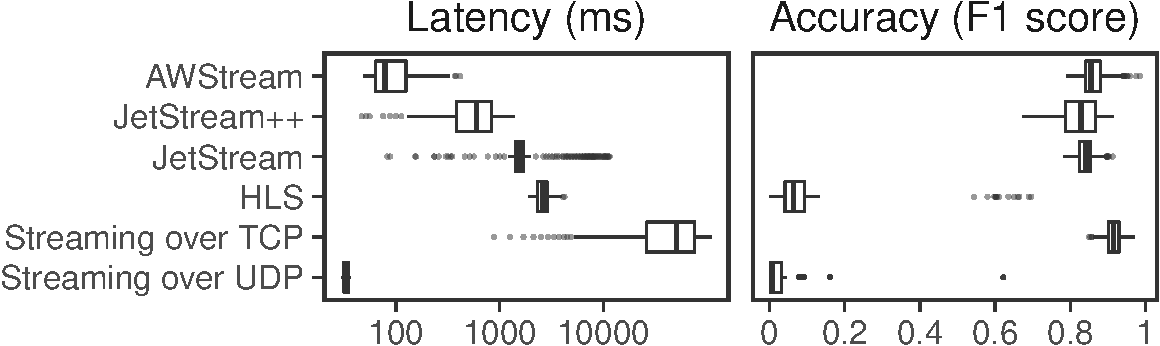
\includegraphics[width=\textwidth]{figures/runtime_mot-boxplot.pdf}
    \begin{picture}(0,0)
      \put(-10, 130){\parbox{2cm}{\centering \caption{PD}\label{fig:pd-runtime}}}
    \end{picture}
  \end{subfigure}
  \\
  \vspace{1em}
  \begin{subfigure}[t]{0.85\textwidth}
    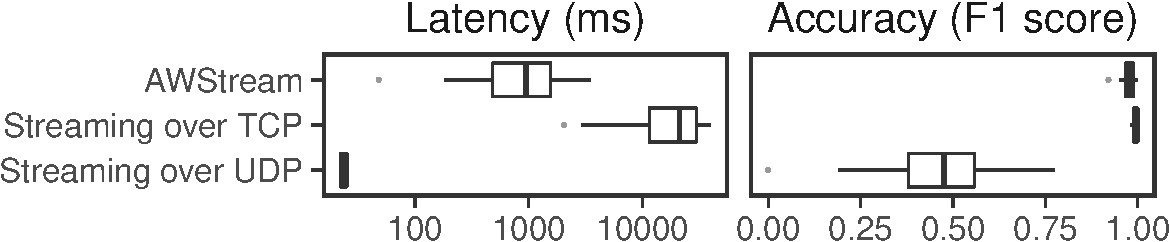
\includegraphics[width=\textwidth]{figures/runtime_tk-boxplot.pdf}
    \begin{picture}(0,0)
      \put(-10, 90){\parbox{2cm}{\centering \caption{TK}\label{fig:tk-runtime}}}
    \end{picture}
  \end{subfigure}
  \caption{PD and TK performance summary. Box plot shows latency and accuracy
    during the traffic shaping (i.e.,~t=200s-440s).}
  \label{fig:pd-tk}
\end{figure}

% \begin{figure}[t]
%   \begin{subfigure}[t]{\columnwidth}
%     \centering
%     \includegraphics[width=\columnwidth]{figures/runtime_mot-timeseries.pdf}
%     \caption{PD's runtime behavior with a time-series plot: throughput (top),
%     showing the effect of bandwidth shaping; latency (middle) in log scale;
%     and accuracy (bottom).}
%     \label{fig:pd-runtime-timeseries}
%   \end{subfigure}
%   \vspace{1em}
%   \\
%   \begin{subfigure}[t]{\columnwidth}
%     \centering
%     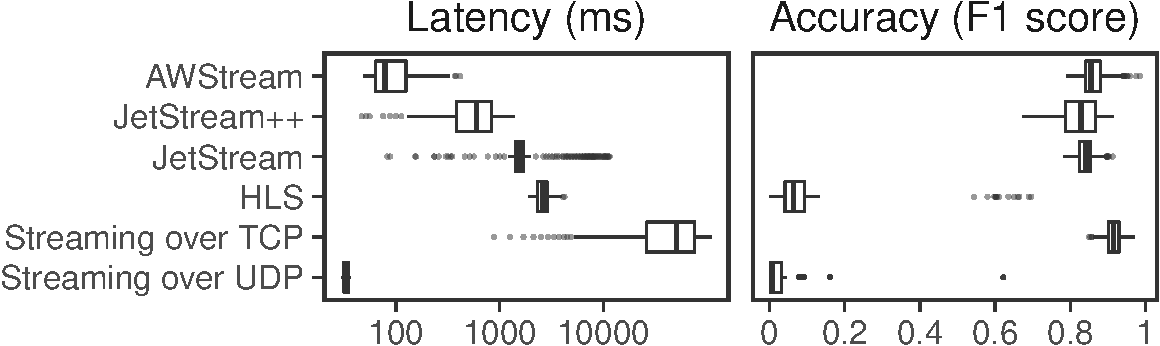
\includegraphics[width=\columnwidth]{figures/runtime_mot-boxplot.pdf}
%     \caption{PD's performance summary of latency and accuracy during the traffic
%     shaping (between t=200s and t=440s).}
%     \label{fig:pd-runtime-boxplot}
%   \end{subfigure}
%   \caption{PD runtime evaluation.}
%   \label{fig:pd-runtime}
%   \vspace{-0.5em}
% \end{figure}

% \begin{figure}[t]
%   \begin{subfigure}[t]{\columnwidth}
%     \centering
%     \includegraphics[width=\columnwidth]{figures/runtime_tk-timeseries.pdf}
%     \caption{TK's runtime behavior with a time-series plot: throughput (top),
%     showing the effect of bandwidth shaping; latency (middle) in log scale;
%     and accuracy (bottom).}
%     \label{fig:tk-runtime-timeseries}
%   \end{subfigure}
%   \vspace{1em}
%   \\
%   \begin{subfigure}[t]{\columnwidth}
%     \centering
%     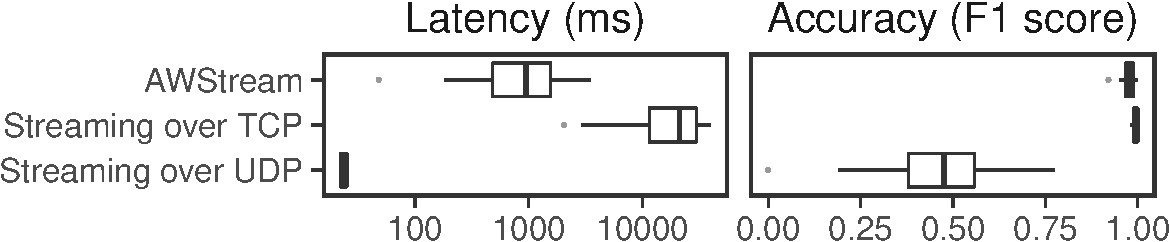
\includegraphics[width=\columnwidth]{figures/runtime_tk-boxplot.pdf}
%     \caption{TK's performance summary of latency and accuracy during the traffic
%     shaping (between t=200s and t=440s).}
%     \label{fig:tk-runtime-boxplot}
%   \end{subfigure}
%   \caption{TK runtime evaluation.}
%   \label{fig:tk-runtime}
%   \vspace{-0.5em}
% \end{figure}

\para{Pedestrian Detection.} The setup for PD is the same with AR: three clients
and one server on EC2. $c_{\max}$ is 1920x1080 resolution, \(10~\text{FPS}\) and
20 quantization; it consumes about \SI{12}{Mbps}. For PD, \awstream{} learns that
resolution is more important than frame rate. Hence it favors 1080p with 10FPS
over 900p with 30FPS. We use the same bandwidth shaping schedule and baselines
as AR. \autoref{fig:pd-runtime} shows the result and most observations about
latency/accuracy are the same as AR. HLS has a poor accuracy because it reduces
resolution and encoding quality during adaptation. \awstream{} is able to achieve
the lowest latency (\SI{78}{ms}) with small accuracy drop (86\%, 6\% drop in
comparison to TCP). In comparison to JetStream, \awstream{} improves the latency
by 20$\times$ (from \SI{1535}{ms} to \SI{78}{ms}) and accuracy by 1\% (from 84\%
to 85\%).

\para{Top-K.} For TK, we use four clients and one server because our logs are
split into four groups. $c_{\max}$ is $N=9750$ for \texttt{head} and $T=0$ for
\texttt{threshold}; it consumes about \SI{1.2}{Mbps}. Because the overall
bandwidth consumption is much smaller than video analytics, we modify the
bandwidth parameter: during t=200-380s, we limit the bandwidth to
\SI{750}{Kbps}; during t=380-440s, the bandwidth is \SI{500}{Kbps}; the
background limit is \SI{2.5}{Mpbs}. We only compared \awstream{} with streaming
over TCP and UDP. JetStream's Top-K is based on TPUT~\cite{cao2004efficient}
that targets at queries asked hourly or daily. We did not implement our Top-K
pipeline (\autoref{fig:topk}) with JetStream because video analytics suffice the
purpose of comparison. \autoref{fig:tk-runtime} shows the evaluation
results. Streaming over TCP has the highest accuracy (99.7\%) but the worst
latency (up to 40 seconds). Streaming over UDP has the lowest latency but the
worst accuracy (52\%). \awstream{} achieves low latency (1.1 seconds) and high
accuracy (98\%) simultaneously. Notice that because TK's source generates data
every second after \texttt{Window}, one object in the queue leads to one second
latency.

\vspace{0.3em}
\para{Performance with Varying Network Delays}

\noindent \awstream{} targets at wide area whose key characteristic is the large
variation in latency~\cite{li2010cloudcmp}. While we have conducted experiments
using real-world setup on EC2, the latency between EC2 sites is relatively low.
To evaluate how \awstream{} performs with increased network delays, we conducted
another experiment with one pair of client and server under different network
conditions. We use \texttt{netem} to add delays, up to \SI{250}{ms} each way, so
the added RTT can be as high as \SI{500}{ms}. The delay follows a normal
distribution where the variation is 10\% (e.g.,~$250\pm 25\text{ms}$).

\begin{figure}
  \centering
  \includegraphics[width=.7\columnwidth]{figures/runtime_darknet-bench.pdf}
  \vspace{0.5em}
  \caption{\awstream{} maintains low latency and high accuracy under different
    network delay conditions.}
  \label{fig:ar-rtt}
\end{figure}

\begin{figure}
  \centering
  \begin{subfigure}[t]{0.6\columnwidth}
    \centering
    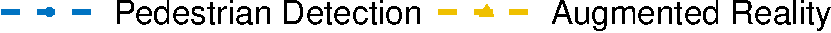
\includegraphics[width=\textwidth]{figures/multitask-legend.pdf}
  \end{subfigure}
  \\\vspace{0.4em}
  \begin{subfigure}[t]{0.45\columnwidth}
    \centering
    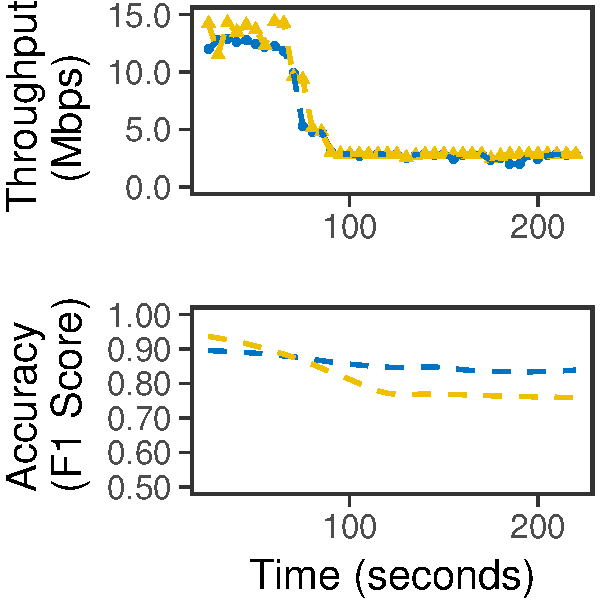
\includegraphics[width=\textwidth]{figures/multitask-left.pdf}
    \caption{Resource Fairness}
    \label{fig:eq-bw}
  \end{subfigure}
  \hfill
  \begin{subfigure}[t]{0.45\columnwidth}
    \centering
    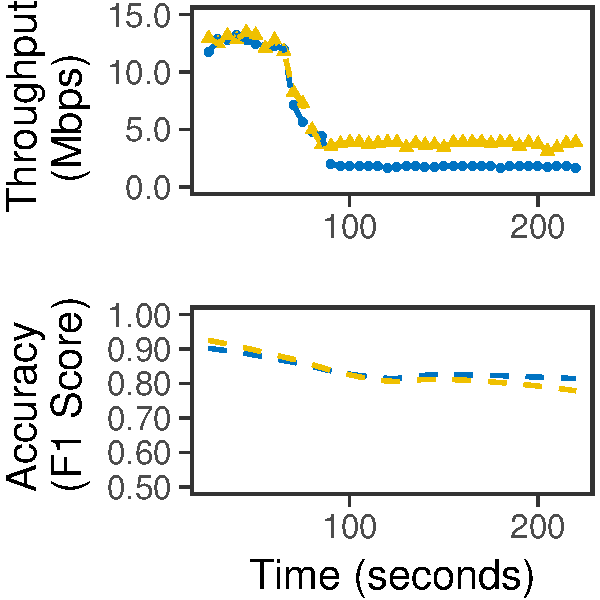
\includegraphics[width=\textwidth]{figures/multitask-right.pdf}
    \caption{Utility Fairness}
    \label{fig:eq-acc}
  \end{subfigure}
  \caption{\awstream{} allows different resource allocation schemes.}
  \label{fig:multitask}
\end{figure}

\autoref{fig:ar-rtt} shows the runtime behavior with various added network
delays. While the latency increases with the added delay, \awstream{} mostly
manages to achieve sub-second latency for all conditions. We see a higher
variation in latency and more outliers as network delay increases, because the
congestion detection is slow when the RTT is high. In terms of accuracy, because
\awstream{} mostly stays in \texttt{Steady} state and accuracy only depends on
the level of degradation, \awstream{} achieves similar accuracy for different
network delays.

\subsection{Resource Allocation and Fairness}
\label{sec:multi-task-alloc}

We evaluate resource allocations with two applications. In this way, the result
also covers the case of a single application, and can generalize to more
applications.

We choose AR and PD as the example applications.  The clients and servers of
both applications are co-located so that they share the same bottleneck
link. The experiment starts with sufficient bandwidth. At t=60s, we start
traffic shaping to limit the total bandwidth to \SI{6}{Mbps}. When we allocate
resource equally between two applications (\autoref{fig:eq-bw}), each
application gets \SI{3}{Mbps}. Under this condition, PD runs with a higher
accuracy of 85\% while AR only achieves 77\%. In addition to resource fairness,
\awstream{} supports utility fairness: it chooses configurations that maximize
the minimal accuracy. In this experiment, PD receives \SI{2}{Mbps} and AR
receives \SI{4}{Mbps}; and both achieve 80\% accuracy (\autoref{fig:eq-acc}).

%%% Local Variables:
%%% mode: latex
%%% TeX-master: "../network"
%%% End:

%% LocalWords: TK PD runtime JetStream AR alloc YOLO dataset outliers
%% LocalWords: makespan subsec mins tcp boxplot geo HLS ffmpeg geforce
%% LocalWords: HLS PD's mis bw quantization RTSP RTP GPUs parallelization
%% LocalWords: eq netem resizes RTTs parallelize LFS UDP GTX analytics
%% LocalWords: FFmpeg GeForce HLS's JetStream's TK's tc HTB TPUT RTT

\subsection{HTTP Live Streaming}
\label{sec:hls}

\begin{figure}[t]
  \centering
  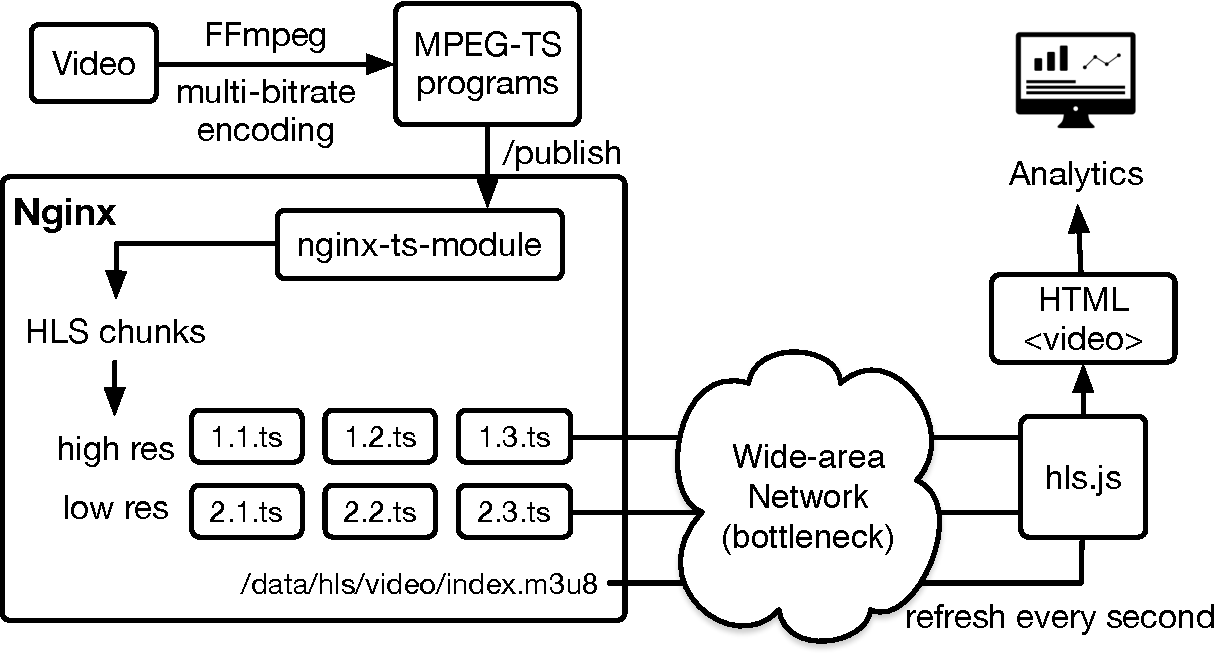
\includegraphics[width=\textwidth]{figures/hls.pdf}
  \caption{HLS setup. (Left) High-level overview: machine 1 generates a video
    and stores it in the server; machine 2 fetches the data and performs
    analytics. (Right) Detailed view: (1)~FFmpeg encodes video with multiple
    bitrates and groups them into MPEG-TS programs; (2)~\texttt{nginx-ts-module}
    then generates HLS chunks on the fly and stores them for nginx serving;
    (3)~the client (using \texttt{hls.js}) periodically fetches the latest index
    file (\texttt{index.m3u8}) and then downloads the right chunk according to
    network conditions.}
  \label{fig:hls-arch}
\end{figure}

HTTP Live Streaming (HLS)~\cite{pantos2016http} represents a class of HTTP-based
media streaming protocols. Other protocols include Adobe HTTP Dynamic
Streaming~\cite{adobestreaming}, Microsoft Smooth
Streaming~\cite{zambelli2009iis}, and a newer vendor-independent standard
DASH~\cite{michalos2012dynamic, sodagar2011mpeg}. These adaptive streaming
protocols are widely adopted for both video-on-demand (VoD) and live streaming
(such as Periscope).

Our setup (\autoref{fig:hls-arch}) resembles the setup of popular live streaming
services~\cite{wang2016anatomy}. We first describe each component of our
setup. We then discuss why these protocols are a poor match for wide-area
streaming analytics, despite their adaptation capability.

\para{Video.} We use \texttt{FFmpeg} to encode the video with multiple bitrates:
all levels use 30FPS, but different resolutions and H.264 encoding quality. Our
experiment uses six different bitrates---900p, 720p, 540p, 360p, all with normal
encoding quality; and 720p, 540p, with low encoding quality. To simulate live
video streaming, we then use \texttt{FFmpeg} to re-publish the stream to an
Nginx web server that accepts MPEG-TS (MPEG transport stream).

\para{Server.} Our web server is a nginx server compiled with plugin
\texttt{nginx-ts-module}~\cite{nginx-ts-module} that receives MPEG-TS over HTTP,
produces live HLS and DASH chunks. It creates an index file \texttt{index.m3u8}
that describes the media stream. During live streaming, the file is updated
whenever new chunks arrive. And the client needs to fetch the newest version of
\texttt{index.m3u8} to find out about new chunks. Typical streaming servers set
each chunk to be 2-10 seconds~\cite{mao2017neural, sun2016cs2p,
  wang2016anatomy}. For our low latency streaming, we configured the chunk
segment to be 1 second.

\para{Analytics.} The HTTP client reads the index file and then fetches each
chunk based on available bandwidth. Our client uses \texttt{hls.js}
\cite{hls.js}, a JavaScript library that implements an HLS client. It directly
plays the video inside an HTML5 video element. To avoid invoking the graphical
front-end of a browser, we use Puppeteer~\cite{puppeteer}, a NodeJS library that
provides a high-level API to control headless Chrome. During the runtime
experiment, instead of playing the video, we record the metadata with each
received chunk: its size, timestamp, and the quality level. We perform an
offline analysis of the log files to calculate the throughput, latency, and
accuracy.

Notice that the client-server relationship is reversed in HLS and \awstream{}. In
HLS, the server hosts video source files; the client fetches videos and
plays/computes. In \awstream{}, the client generates videos and pushes frames to
the server; the server performs video analytics.

\vspace{0.5em}
\para{Why HLS/DASH is a poor match for video analytics?} It's hard to achieve
ultra low latency using HLS/DASH: (1) HLS/DASH is pull-based: the client keeps
requesting for new chunks; (2) HLS/DASH uses chunking: shorter chunks enable a
lower latency, but induce a larger number of requests, and the chunk has to be
made ready before the client can start fetching. There are proposals to reduce
the latency, such as server push~\cite{wei2014low}, but they are still work in
progress. For some applications, the accuracy can also be poor if these videos
are limited to tuning resolution and encoding quality only, as demonstrated by
in our PD evaluation.

%%% Local Variables:
%%% mode: latex
%%% TeX-master: "../network"
%%% End:

\subsection{JetStream++}
\label{sub:jetstream++}

We modified the open source version of
JetStream\footnote{\url{https://github.com/princeton-sns/jetstream/}, \newline
  commit bf0931b2d74d20fdf891669188feb84c96AF84.} in order to use our profile as
its manual policy. Because JetStream doesn't support simultaneous degradation
across multiple operators, we implemented a simple \texttt{VideoSource} operator
that understands how to change image resolutions, frame rate, and video encoding
quantization. At runtime, \texttt{VideoSource} queries congestion policy manager
and adjusts three dimensions simultaneously. This operator is then exposed to
the Python-implemented control plane. We call this modified version
JetStream++.\footnote{\url{https://github.com/awstream/jetstream-clone/pull/1}}

JetStream's code base is modular and extensible: the modifications include 53
lines for the header file, 171 lines for implementation, 75 lines for unit test,
and 49 lines of python as the application. While extending JetStream with our
profile is not challenging, JetStream++ performs degradation in a single
operator and loses the composability. We could modify JetStream to support
degradation across multiple operators, but that would require substantial
changes to JetStream. Using JetStream++ with our profile, the comparison is
enough to illustrate the difference between \awstream{}'s and JetStream's
runtime.

%%% Local Variables:
%%% mode: latex
%%% TeX-master: "../network"
%%% End:

%% LocalWords: Mbps analytics runtime JetStream OpenCV YOLO pre GStreamer appsrc
%% LocalWords: appsink zerolatency quantization dataset SVM geo topk VideoSource
%% LocalWords: JetStream's composability TK TCP UDP HLS FFmpeg bitrates nginx
%% LocalWords: packetization TPUT topk NodeJS metadata timestamp Mbps Kbps
%% LocalWords: aws PD's TK's hls js VoD awstream tk fdf feb

\section{Discussion and Future work}
\label{sec:discussion}

\paraf{Reducing Developer Effort.} While \awstream{} simplifies developing
adaptive applications, there are still application-specific parts required for
developers: wrapping appropriate \maybe{} calls, providing training data, and
implementing accuracy functions. Because \awstream{}'s API is extensible, we plan
to build libraries for common degradation operations and accuracy functions,
similar to machine learning libraries.

\para{Fault-tolerance and Recovery.} \awstream{} tolerates bandwidth variation
but not network partition or host failure. Although servers within data centers
can handle faults in existing systems, such as Spark
Streaming~\cite{zaharia2013discretized}, it is difficult to make edge clients
failure-oblivious.  We leave failure detection and recovery as a future work.

\para{Profile Modeling.} \awstream{} currently performs an exhaustive search when
profiling. While parallelism and sampling are effective, profiling complexity
grows exponentially with the number of knobs. Inspired by recent success of
using Bayesian Optimization~\cite{snoek2012practical, alipourfard2017cherrypick,
  solnik2017bayesian} to model black-box functions, we are currently exploring
multi-objective Bayesian Optimization~\cite{hernandez2016predictive} that can
find \textit{near-optimal} configurations without exhaustive search.

% \para{Expressiveness}: Our \maybe{} APIs allow an easy integration with
% existing stream processing systems. While it follows the operator model,
% combined with other operators, this is expressive enough. We've presented
% three applications in this paper; and we are implement more application using
% this framework to understand the expressiveness better.

\para{Context detection.} \awstream{} is currently limited to one profile: the
offline profiling generates the default profile and the online profiling
updates the single profile continuously.  Real-world applications may produce
data with a multi-modal distribution, where the model changes upon context
changes, such as indoor versus outdoor. Therefore, one possible optimization
to \awstream{} is to allow multiple profiles for one application, detect
context changes, and use the profile that best matches the current data
distribution.  Switching contexts could reduce, or even eliminate, the
overhead of online profiling.

\para{Bandwidth Estimation and Prediction.} Accurately estimating and predicting
available bandwidth in wide area remains a challenge~\cite{huang2012confused,
  zou2015can}. \awstream{} uses network throughput and behaves cautiously to
avoid building up queues: congestion is detected at both sender/receiver; data
rate only increases after probing.  Recent research on adaptive video streaming
explores model predictive control (MPC)~\cite{yin2015control, sun2016cs2p} and
neural network~\cite{mao2017neural}. We plan to explore these techniques next.

%%% Local Variables:
%%% mode: latex
%%% TeX-master: "../network"
%%% End:

%% LocalWords: CherryPick runtime MPC QoE profiler

\section{Chapter Summary}
\label{sec:chapter-summary}

The emerging class of wide-area streaming analytics faces the challenge of
scarce and variable bandwidth. Developers need to make a trade-off between data
freshness and fidelity. While it is easy to build applications for either high
accuracy or low latency, achieving both simultaneously is challenging. Previous
approaches using manual policies end up with sub-optimal
performance. Application-specific optimizations do not generalize to cover the
variety and scales of potential applications.

This chapter presents \awstream{}, a stream processing system for a wide variety
of applications by enabling developers to customize degradation operations with
\maybe{} operators. Our automatic profiling tool generates an accurate profile
that characterizes the trade-off between bandwidth consumption and application
accuracy. The profile allows the runtime to react with precision. Evaluations
with three applications show that \awstream{} achieves sub-second latency with
nominal accuracy drop. \awstream{} enables resilient execution of wide-area
streaming analytics with minimal developer effort.

%%% Local Variables:
%%% mode: latex
%%% TeX-master: "../network"
%%% End:

%% LocalWords: analytics runtime


\end{document}

%%% Local Variables:
%%% mode: latex
%%% TeX-master: t
%%% End:
